\documentclass[12pt,a4paper]{report}
\usepackage[english]{babel}
\usepackage{newlfont}
\usepackage{physics}
\usepackage{amsmath}
\usepackage{amssymb}
\usepackage{amsthm}
\usepackage{xcolor}
\usepackage{listings}
\usepackage{tikz}
\usepackage{xspace}
\usepackage[
backend=biber,
style=alphabetic,
sorting=ynt
]{biblatex}


\addbibresource{bibliography.bib}


\usetikzlibrary{quantikz}
\usetikzlibrary{shapes}
\usetikzlibrary{shapes.multipart}


\theoremstyle{definition}
\newtheorem{definition}{Definition}[section]

\theoremstyle{definition}
\newtheorem{example}{Example}[section]

\theoremstyle{definition}
\newtheorem{problem}{Problem}[section]

\textwidth=450pt\oddsidemargin=0pt
\newenvironment{dedication}
{%\clearpage           % we want a new page          %% I commented this
\thispagestyle{empty}% no header and footer
\vspace*{\stretch{1}}% some space at the top
\itshape             % the text is in italics
\raggedleft          % flush to the right margin
}
{\par % end the paragraph
\vspace{\stretch{3}} % space at bottom is three times that at the top
\clearpage           % finish off the page
}

\lstset{% This applies to ALL lstlisting
  basicstyle=\small\ttfamily\color{black},%
  breaklines=true,%
  numbers=none,
  moredelim=[s][\color{green!50!black}\ttfamily]{'}{'},% single quotes in green
}%








\begin{document}
\begin{titlepage}
\begin{center}
{{\Large{\textsc{Alma Mater Studiorum $\cdot$ Universit\`a di
Bologna}}}} \rule[0.1cm]{15.8cm}{0.1mm}
\rule[0.5cm]{15.8cm}{0.6mm}
{\small{\bf SCUOLA DI SCIENZE\\
Corso di Laurea in Informatica }}
\end{center}
\vspace{15mm}
\begin{center}
{\LARGE{\bf Static Analysis of Resources in QASM:}}\\
\vspace{3mm}
{\LARGE{\bf Estimation of the Number of Qubits}}\\
\end{center}
\vspace{40mm}
\par
\noindent
\begin{minipage}[t]{0.47\textwidth}
{\large{\bf Relatore:\\
Chiar.mo Prof.\\
Ugo Dal Lago\\
}}
\end{minipage}
\hfill
\begin{minipage}[t]{0.47\textwidth}\raggedleft
{\large{\bf Presentata da:\\
Damiano Scevola}}
\end{minipage}
\vspace{20mm}
\begin{center}
{\large{\bf Sessione I\\%inserire il numero della sessione in cui ci si laurea
Anno Accademico 2020/2021}}%inserire l'anno accademico a cui si è iscritti
\end{center}
\end{titlepage}

\begin{dedication}
A nonno Francesco
\end{dedication}

\tableofcontents



\chapter{Introduction}
The idea of quantum computing was conceived in the 1970s, when researchers of the caliber of Feynman, Manin and Deustch started to theorize that the properties of quantum mechanics might prove useful for performing computations differently from the classical paradigm \cite{zuw}. The main concept that lays at the core of this new model is the superposition of states, that is the simultaneous co-existence of multiple computational states at the same moment, with the possibility to perform the same operation to all of those states with a single computational step. Physical devices that are capable of such power are called ``quantum computers'', and they constitute a polynomial-time implementation of non-determinism, thus achieving an exponential-order level of parallelism. This fact invalidates the assumption that some problems (NP-complete ones, for instance) require too much time to be solved compared to human life duration, hence it opens the doors to a new variety of applications, and it also tears down the ones which rely on this assumption (like RSA cryptography). Literature usually refers to this scenario as ``Quantum Supremacy''.\\
Quantum computers operate through qubits, which are the quantum equivalent of bits, and can have not only $0$s and $1$s as values, but also combinations of them. Qubits are sequenced together to form quantum registers, which hold the actual computational power of quantum computers. For instance, a 3-qubit register can be in a superposition of the states $\ket{000}, \ket{001}, \ket{010}, \ldots, \ket{111}$, that are $2^3=8$ base states. Generalizing the previous result, we notice that an $n$-qubit register can represent up to $2^n$ states simultaneously, thus showing where the exponential speedup resides.\\
Some companies like Google and IBM have already built fully-functional quantum computers. However, all of them have a limited number of qubits due to the elevate cost of implementing them physically. Therefore, it is crucial that quantum programmers are thrifty with the usage of qubits while designing quantum circuits. The aim of this document is to show a simple tool which is able to analyze programs written in QASM language (Quantum Assembly) and check whether the number of qubits that are \textit{effectively} used is bounded by a certain expression.
We start by introducing some concepts of quantum computing, then we describe the QASM language and we provide details about the features that are taken into account by the analyzer. Finally we describe the tool that performs the estimation of the number of qubits by presenting the modules APIs it is built upon one by one, and in the last chapter we discuss how the estimation of the number of qubits is actually performed, going through some examples.\\



\chapter{Quantum Computing}


\section{Quantum states}
\subsection{Deterministic systems}
In classical systems, when we need to encode the state of an object, we often use numbers. For example, consider a simple case where we have a skyscraper with $n$ floors (counting the ground floor also), and we want to represent on which one an employee is located. Trivially, this can be done using an integer number $k$, and if we assume there are no underground floors, then we can state $k \in \{0, 1, \ldots, n-1\}$.\\
Another option for representing such a state would be using a \textit{state vector}, that is a vector $\mathbf{v}\in\{0,1\}^n$ whose entries are all zeros except for the $k$-th, which is a $1$.
\begin{center}
\begin{tikzpicture}
\draw (0,0) -- (0,-6);
\draw (8,0) -- (8,-6);

\filldraw[black] (0,0) circle (2pt) node[anchor=west] {$n-1$};
\filldraw[black] (0,-1) circle (2pt) node[anchor=west] {$n-2$};
\filldraw[black] (0,-2) circle (0pt) node[anchor=west] {$\vdots$};
\filldraw[black] (0,-3) circle (3pt) node[anchor=west] {$k$};
\filldraw[black] (0,-4) circle (0pt) node[anchor=west] {$\vdots$};
\filldraw[black] (0,-5) circle (2pt) node[anchor=west] {$1$};
\filldraw[black] (0,-6) circle (2pt) node[anchor=west] {$0$};

\filldraw[black] (8,-0) circle (2pt) node[anchor=west] {$0$};
\filldraw[black] (8,-1) circle (2pt) node[anchor=west] {$0$};
\filldraw[black] (8,-2) circle (0pt) node[anchor=west] {$\vdots$};
\filldraw[black] (8,-3) circle (3pt) node[anchor=west] {$1$};
\filldraw[black] (8,-4) circle (0pt) node[anchor=west] {$\vdots$};
\filldraw[black] (8,-5) circle (2pt) node[anchor=west] {$0$};
\filldraw[black] (8,-6) circle (2pt) node[anchor=west] {$0$};
\end{tikzpicture}
\end{center}
Such an approach seems exaggerated for this simple case, but it is crucial to understand how quantum systems work. Let's take a look at another scenario.




\subsection{Probabilistic systems}
Imagine now that the floor the employee is on is not known for sure, but we are only given probabilities of her being on each floor. The state vector now looks something like:
\begin{equation*}
    \mathbf{v}=\begin{bmatrix}
        p_0\\
        p_1\\
        \vdots\\
        p_{n-1}\\
    \end{bmatrix}\in [0,1]^n
\end{equation*}
We now have a generalized version of our previously defined state vector, because each entry $p_i$ is a real number between $0$ and $1$. Since we are talking about probabilities, we set the constraint that all the entries of $\mathbf{v}$ must sum up to $1$.
\begin{equation*}
    \sum_{i=0}^{n-1} p_i = 1
\end{equation*}
It should be noticed that there is no way to represent probabilistic states with a single number like we do for deterministic ones. It is clear, however, that in case we know the exact location of the employee, the vector would collapse to the previous case. In fact, if we are certain that the employee is on the $k$-th floor, then $p_k=1$, and $\forall i \in \{0,1,\ldots,n-1\} \smallsetminus \{k\},\ p_i=0$.\\
Now it is time to define state vectors for quantum systems.\\




\subsection{Quantum systems}
Consider a quantum object (e.g. an electron or a photon), and assume its position can be measured in the domain $\{x_1, x_2, \ldots, x_n\}$.\\
\begin{center}
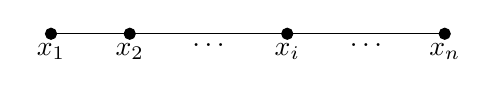
\begin{tikzpicture}
\draw (0,0) -- (5,0);
\filldraw[black] (0,0) circle (2pt) node[anchor=north] {$x_1$};
\filldraw[black] (1,0) circle (2pt) node[anchor=north] {$x_2$};
\filldraw[black] (2,0) circle (0pt) node[anchor=north] {$\ldots$};
\filldraw[black] (3,0) circle (2pt) node[anchor=north] {$x_i$};
\filldraw[black] (4,0) circle (0pt) node[anchor=north] {$\ldots$};
\filldraw[black] (5,0) circle (2pt) node[anchor=north] {$x_n$};
\end{tikzpicture}
\end{center}

To each position $x_i$, it corresponds a basic vector having as entries all zeros and a $1$ as the $i$-th entry.
\begin{equation*}
    \ket{x_1} = \begin{bmatrix}
        1\\
        0\\
        \vdots\\
        0\\
    \end{bmatrix},\ 
    \ket{x_2} = \begin{bmatrix}
        0\\
        1\\
        \vdots\\
        0\\
    \end{bmatrix},\ \ldots,\ 
    \ket{x_n} = \begin{bmatrix}
        0\\
        0\\
        \vdots\\
        1\\
    \end{bmatrix}
\end{equation*}

\begin{definition}[Quantum State]
A quantum state $\ket{\psi}$ is a linear combination of the basic vectors $\ket{x_1}, \ket{x_2}, \ldots, \ket{x_n}$ having complex weights $c_1, c_2, \ldots, c_n \in \mathbb{C}$.
\begin{equation*}
    \ket{\psi}=c_1\ket{x_1}+c_2\ket{x_2}+\cdots+c_n\ket{x_n}
\end{equation*}
Therefore, $\ket{\psi}$ can be represented as
\begin{equation*}
    \ket{\psi}=\begin{bmatrix}
        c_0\\
        c_1\\
        \vdots\\
        c_{n-1}\\
    \end{bmatrix}\in \mathbb{C}^n
\end{equation*}
where
\begin{equation*}
    \sum_{i=0}^{n-1} \left\lvert c_i \right\rvert ^2 = 1
\end{equation*}
\end{definition}
Since it is a weighted sum of basic states, we say that $\ket{\psi}$ is a \textit{superposition} of the basic states.
The square norm of $c_i$ tells us the probability of observing the particle in the position $x_i$, and since the particle is indeed in one of those positions, the sum of square norms must add up to $1$.\\
The reason why we need complex numbers to represent quantum states is that quantum objects (like photons or electrons) behave both like particles and waves, so they can interfere either constructively or disruptively. By using complex numbers, we can sum waves and capture the fact that they could interfere disruptively, since the square norm of the sum of two complex number is not necessarily greater than both of the square norms of the addends.



\section{Qubits and quantum registers}
\subsection{Bits and qubits}
In order to understand what qubits are, we should remark the meaning of classical bits and then make a generalization.
\begin{definition}[Bit]
A bit is an elementary unit of information describing the state of the simplest classical system.
\end{definition}
As we know, a bit can only assume values in the domain $\{0,1\}$.
\begin{center}
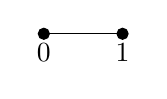
\begin{tikzpicture}
\draw (0,0) -- (1,0);
\filldraw[black] (0,0) circle (2pt) node[anchor=north] {$0$};
\filldraw[black] (1,0) circle (2pt) node[anchor=north] {$1$};
\end{tikzpicture}
\end{center}
By following the approach of the previous section, we can also describe bits using a two-dimensional state vector, where the first element stands for $0$, and the last for $1$:
\begin{equation*}
    \ket{0}=\begin{bmatrix}
        1\\
        0
    \end{bmatrix},\ 
    \ket{1}=\begin{bmatrix}
        0\\
        1
    \end{bmatrix}
\end{equation*}
If we take $\ket{0}$ and $\ket{1}$ as basic states, we can define a quantum system by considering all normalized linear combinations of those states. Such a quantum system is called \textit{qubit}.
\begin{definition}[Qubit]
A qubit is a quantum system having $\ket{0}$ and $\ket{1}$ as basic states, and therefore it can be represented as an element of $\mathbb{C}^2$.
\begin{equation*}
    \ket{q}=c_0\ket{0}+c_1\ket{1}=c_0\begin{bmatrix}
        1\\
        0
    \end{bmatrix}+c_1\begin{bmatrix}
        0\\
        1
    \end{bmatrix}=\begin{bmatrix}
        c_0\\
        c_1
    \end{bmatrix} \in \mathbb{C}^2
\end{equation*}
Keep in mind that the sum of the square norms must be equal to $1$. In other words, the state must be \textit{normalized}.
\begin{equation*}
    \left|c_0\right|^2+\left|c_1\right|^2=1
\end{equation*}
\end{definition}
\begin{example}
Here is an example of a qubit:
\begin{equation*}
    \ket{q}=\frac{\ket{0}+\ket{1}}{\sqrt{2}}=\begin{bmatrix}
        \frac{1}{\sqrt{2}}\\
        \frac{1}{\sqrt{2}}
    \end{bmatrix}
\end{equation*}
In fact, if we check the sum of the square norms of the coefficients, we see that they add up to $1$.
\begin{equation*}
    \left(\frac{1}{\sqrt{2}}\right)^2+\left(\frac{1}{\sqrt{2}}\right)^2=\frac{1}{2}+\frac{1}{2}=1
\end{equation*}
Of course, the following are also qubits:
\begin{equation*}
    \ket{q_0}=\frac{\ket{0}-\ket{1}}{\sqrt{2}}=\begin{bmatrix}
        \frac{1}{\sqrt{2}}\\
        -\frac{1}{\sqrt{2}}
    \end{bmatrix},\ 
    \ket{q_1}=\frac{\ket{1}-\ket{0}}{\sqrt{2}}=\begin{bmatrix}
        -\frac{1}{\sqrt{2}}\\
        \frac{1}{\sqrt{2}}
    \end{bmatrix}
\end{equation*}
\end{example}
We shall notice that $\ket{q}$, $\ket{q_0}$ and $\ket{q_1}$ are all superpositions of the basic states $\ket{0}$ and $\ket{1}$.




\subsection{Measurement}
When we measure a qubit, the possible outcomes are only $0$ and $1$, and the probability of observing the one or the other is dictated by the square norms of the coefficients $c_0$ and $c_1$. In addition to this, the measurement affects the internal state of the qubit permanently, making it collapse to the value that has just been measured.
\begin{example}
Consider a qubit whose state is
\begin{equation*}
    \ket{\psi}=\frac{\sqrt{3}}{2}\ket{0}+\frac{1}{2}\ket{1}
\end{equation*}
If we measure it, we have $\left(\frac{\sqrt{3}}{2}\right)^2=\frac{3}{4}=75\%$ of probability to observe the outcome being $0$, and $\left(\frac{1}{2}\right)^2=\frac{1}{4}=25\%$ of probability of it being $1$.\\
Let's say we obtained $0$ from the measurement. The state of the qubit is not $\ket{\psi}$ anymore, but it has become $\ket{\psi'}=\ket{0}$ because the measurement made it collapse as a side effect, so if we measure it again we have $100\%$ of chances to observe the value $0$ again.\\
This fact is at the core of quantum mechanics, and it just tells us that in order to observe something we must inevitably interact with it and alter its internal state.
\end{example}




\subsection{Quantum registers}
Quantum computers with a single qubit are not very interesting, so we need a way to combine qubits and form registers. In order to combine quantum systems, we need to use the tensor product.
For example, let's say we wanted to represent the two-qubits state $\ket{01}$. We would then need to compute the tensor product $\ket{0}\otimes\ket{1}$ as follows:
\begin{equation*}
    \ket{0}\otimes\ket{1}=\begin{bmatrix}
        1\\
        0
    \end{bmatrix}\otimes\begin{bmatrix}
        0\\
        1
    \end{bmatrix}=\begin{bmatrix}
        1\begin{bmatrix}
            0\\
            1
        \end{bmatrix}\\
        0\begin{bmatrix}
            0\\
            1
        \end{bmatrix}
    \end{bmatrix}=\begin{bmatrix}
            0\\
            1\\
            0\\
            0
    \end{bmatrix}=\begin{bmatrix}
            c_{00}\\
            c_{01}\\
            c_{10}\\
            c_{11}
    \end{bmatrix}
\end{equation*}
If we observe the result carefully, we can notice that the normalization constraint still holds, and the only $1$ that appears in the final result corresponds to $c_{01}$, which is right the coefficient labelled with our state $\ket{01}$. If we try to do the same thing with the state $\ket{101}$, we will obtain:
\begin{equation*}
    \ket{101}=\ket{1}\otimes\ket{0}\otimes\ket{1}=\begin{bmatrix}
        0\\
        0\\
        0\\
        0\\
        0\\
        1\\
        0\\
        0
    \end{bmatrix}=\begin{bmatrix}
        c_{000}\\
        c_{001}\\
        c_{010}\\
        c_{011}\\
        c_{100}\\
        c_{101}\\
        c_{110}\\
        c_{111}
    \end{bmatrix}
\end{equation*}
Since the result of the tensor product enumerates all possible states with $n$ qubits, the dimension of the output is as large as $2^n$.\\
Of course, considering the fact that quantum computers allow superpositions of many states, we shall clarify that the previous examples have only taken into account basic states. Hence we can also have a 3-qubit register in the state
\begin{equation*}
    \ket{\psi}=\frac{\ket{000}+\ket{010}-\ket{011}-\ket{100}+\ket{110}}{\sqrt{5}}
\end{equation*}



\subsection{Entanglement}
When multiple qubits are involved to form a quantum register, it can sometimes have the property that if we measure one of the qubits, then we automatically know the value of the others. We say, then, that those qubits are \textit{entangled}.
\begin{example}
Consider a quantum register with 2 qubits and assume its state is
\begin{equation*}
    \ket{\psi}=\frac{\ket{00}+\ket{11}}{\sqrt{2}}
\end{equation*}
Then, if we measure the first qubit and we observe the value $1$, we automatically know that the other qubit also has value $1$ by just noticing that the only basic state that appears in $\ket{\psi}$ and has a $\ket{1}$ at the first position is $\ket{11}$, so we know for sure that the other one is $\ket{1}$ too.\\
In this case, the measurement not only affects the state of the measured qubit making it collapse to $\ket{1}$, but it also collapses the state of the entangled one.
\end{example}




\section{Quantum Gates}
So far we have discussed how to represent qubits and quantum registers and what their properties are, but in order to perform a computation we need a way to manipulate them according to an algorithm and exploit their computational power.\\
Just like classical computers manipulate bits using logic gates, quantum computers use quantum gates to achieve their objective.\\
The physical implementation of quantum gates is as complicated as that of qubits, but we can represent what these gates do by using mathematical objects that operate on state vectors and keep the output normalized so that the sum of the square norms of the coefficients of the output vector is always $1$. These objects are unitary matrices.\\
There are infinite possible quantum gates. Here we describe the set of universal ones $\{H, CNOT, R(\theta)\}$, which includes three gates that can be combined together to simulate an arbitrary gate.\\




\subsection{Hadamard gate}
The Hadamard gate is encoded by the following matrix:
\begin{equation*}
    H=\begin{bmatrix}
        \frac{1}{\sqrt{2}} & \frac{1}{\sqrt{2}} \\
        \frac{1}{\sqrt{2}} & -\frac{1}{\sqrt{2}} \\
    \end{bmatrix}=\frac{1}{\sqrt{2}}\begin{bmatrix}
        1 & 1 \\
        1 & -1
    \end{bmatrix}
\end{equation*}
The Hadamard matrix is the transition matrix from the canonical basis $\left\{\begin{bmatrix} 1 \\ 0\end{bmatrix}, \begin{bmatrix} 0 \\ 1\end{bmatrix}\right\}$ to the Hadamard basis $\left\{\begin{bmatrix} \frac{1}{\sqrt{2}} \\ \frac{1}{\sqrt{2}}\end{bmatrix}, \begin{bmatrix} \frac{1}{\sqrt{2}} \\ -\frac{1}{\sqrt{2}}\end{bmatrix}\right\}$, which is used to express arbitrary states in terms of superpositions of basic states, and this allows calculations to be performed on a superposition, hence on all of the basic states it is composed of with a single computational step.\\
Since $H$ is unitary, by applying it twice we go back to the canonical basis, so after calculations are finished, Hadamard gate can be applied again to translate the results back into the canonical basis, ready to be measured by the observer.
\begin{example}
By applying Hadamard gate to the qubits $\ket{0}$ and $\ket{1}$ we get:
\begin{equation*}
    H\ket{0}=\begin{bmatrix}
        \frac{1}{\sqrt{2}} & \frac{1}{\sqrt{2}} \\
        \frac{1}{\sqrt{2}} & -\frac{1}{\sqrt{2}}
    \end{bmatrix}\begin{bmatrix}
        1 \\
        0
    \end{bmatrix}=\begin{bmatrix}
        \frac{1}{\sqrt{2}} \\
        \frac{1}{\sqrt{2}}
    \end{bmatrix}=\frac{\ket{0}+\ket{1}}{\sqrt{2}}=\ket{+}
\end{equation*}
\begin{equation*}
    H\ket{1}=\begin{bmatrix}
        \frac{1}{\sqrt{2}} & \frac{1}{\sqrt{2}} \\
        \frac{1}{\sqrt{2}} & -\frac{1}{\sqrt{2}}
    \end{bmatrix}\begin{bmatrix}
        0 \\
        1
    \end{bmatrix}=\begin{bmatrix}
        \frac{1}{\sqrt{2}} \\
        -\frac{1}{\sqrt{2}}
    \end{bmatrix}=\frac{\ket{0}-\ket{1}}{\sqrt{2}}=\ket{-}
\end{equation*}
It is easy to verify that applying Hadamard on $\ket{+}$ and $\ket{-}$ we go back respectively to $\ket{0}$ and $\ket{1}$.\\
We will represent the Hadamard gate as a box labelled with `H'\\\\
\begin{quantikz}
    & \lstick{$\ket{0}$} & \gate{H} & \rstick{$\frac{\ket{0}+\ket{1}}{\sqrt{2}}$}\qw&\\
\end{quantikz}\\
\end{example}





\subsection{Controlled NOT gate}
While Hadamard gate affects a single qubit, the controlled NOT gate (CNOT or CX for short) needs two of them. One is the control qubit, and the other is the target.
\begin{quantikz}\\
\lstick{$\ket{x}$} & \ctrl{1} & \rstick{$\ket{x}$} \qw& \\
\lstick{$\ket{y}$} & \targ{} & \rstick{$\ket{x\oplus y}$} \qw& \\
\end{quantikz}\\
Here $\oplus $ denotes the binary exclusive OR operation. That is, if $\ket{x} = \ket{0}$ then the bottom output will be left unaltered, otherwise if $\ket{x} = \ket{1}$, then the bottom qubit is flipped.
The matrix that corresponds to the CNOT gate is:
\begin{equation*}
    \prescript{C}{}{X} = \begin{bmatrix}
    1 & 0 & 0 & 0\\
    0 & 1 & 0 & 0\\
    0 & 0 & 0 & 1\\
    0 & 0 & 1 & 0
    \end{bmatrix}
\end{equation*}




\subsection{Phase shift gate}
Phase shift gate is a parametric gate that affects a single qubit by rotating it in the Bloch sphere, adjusting its phase. We will not go over the details of Bloch sphere representation, but we just give the matrix which encodes the phase shift here.
\begin{equation*}
    R(\theta) = \begin{bmatrix}
        1 & 0 \\
        0 & e^\theta
    \end{bmatrix}
\end{equation*}
Now that we have discussed quantum gates, we can move to designing quantum circuits (or algorithms).





\section{Quantum Circuits}
Quantum circuits are the equivalent of algorithms for classical computing. By combining quantum gates, we can build a circuit that performs a certain computation and exploits the power of superpositions to drastically reduce the time of execution compared to a classical program.
\begin{definition}[Quantum circuit]
A quantum circuit is a computational routine consisting of coherent quantum operations on quantum data, such as qubits, and concurrent real-time classical computation \cite{qsk}. It is an ordered sequence of quantum gates, measurements and resets, all of which may be conditioned on and use data from the real-time classical computation.
\end{definition}
In order to understand how quantum circuits work, we will discuss the Deutsch algorithm for balanced and constant function classification.





\subsection{Deutsch algorithm}
Before describing the Deutsch algorithm, let's define what balanced and constant functions are.
\begin{definition}[Balanced and constant functions]
A function $f: \{0,1\} \longrightarrow \{0,1\}$ is \textit{balanced} if $f(0)\neq f(1)$, otherwise it is \textit{constant}.
\end{definition}
The Deutch algorithm solves the following problem:
\begin{problem}[Deutsch-Jozsa]
Suppose we have a function $f: \{0,1\} \longrightarrow \{0,1\}$ which we can evaluate, but we do not know its exact definition. Determine whether $f$ is balanced or constant.
\end{problem}
If we wanted to use the classical approach, we would need to evaluate $f$ twice and compare the results. With the Deutsch algorithm, we will see that only one evaluation is sufficient.\\
Suppose we have a unitary matrix $U_f$ that encodes $f$:\\
\begin{quantikz}\\
    & \lstick{$\ket{x}$} & \qw & \qw & \gate[wires=2][2cm]{U_f}& \qw & \qw & \rstick{$\ket{x}$}\qw\\
    & \lstick{$\ket{y}$} & \qw & \qw & & \qw & \qw & \rstick{$\ket{y \oplus f(x)}$}\qw\\
\end{quantikz}\\
Let's now build a circuit that uses $U_f$ and solves our problem:\\
\begin{quantikz}\\
    & \lstick{$\ket{0}$} & \qw & \gate{H} & \qw & \gate[wires=2][2cm]{U_f}& \qw & \gate{H} & \qw & \meter{}\\
    & \lstick{$\ket{1}$} & \qw & \gate{H} & \qw &  & \qw & \qw & \qw & \qw &\\
    & & \text{$\ket{\psi_0}$} &  & \text{$\ket{\psi_1}$}  &  & \text{$\ket{\psi_2}$} &  &   \text{$\ket{\psi_3}$} &  &\\
\end{quantikz}\\
In terms of matrices, the circuit corresponds to
\begin{equation*}
    (H \otimes I)U_f(H \otimes H)\ket{0,1}
\end{equation*}
The algorithm starts with the state
\begin{equation*}
    \ket{\psi_0} = \ket{0, 1}
\end{equation*}
Then it proceeds by applying Hadamard to both qubits, putting them in a superposition:
\begin{equation*}
    \ket{\psi_1} = \ket{+,-} = \left[\frac{\ket{0}+\ket{1}}{\sqrt{2}}\right]\left[\frac{\ket{0}-\ket{1}}{\sqrt{2}}\right]=\frac{\ket{0,0}-\ket{0,1}+\ket{1,0}-\ket{1,1}}{2}
\end{equation*}
Now let's pause for a moment and ponder about what happens if we apply $U_f$ to a generic state $\ket{x, -}$.
\begin{equation*}
    U_f\ket{x,-}=U_f(\ket{x}\left[\frac{\ket{0}-\ket{1}}{\sqrt{2}}\right])=U_f\left[\frac{\ket{x,0}-\ket{x,1}}{\sqrt{2}}\right]=\ket{x}\left[\frac{\ket{0 \oplus f(x)}-\ket{1 \oplus f(x)}}{\sqrt{2}}\right]
\end{equation*}
Which simplifies to
\begin{equation*}
    U_f\ket{x,-}=\ket{x}\left[\frac{\ket{f(x)}-\ket{\overline{f(x)}}}{\sqrt{2}}\right]
\end{equation*}
Where we denoted the opposite of $f(x)$ with $\overline{f(x)}$. So we have
\begin{equation*}
    U_f\ket{x,-}=\begin{cases}
        \ket{x}\left[\frac{\ket{0}-\ket{1}}{\sqrt{2}}\right] & if\ f(x) = 0\\
        \ket{x}\left[\frac{\ket{1}-\ket{0}}{\sqrt{2}}\right] & if\ f(x) = 1\\
    \end{cases}
\end{equation*}
We can write the last expression as
\begin{equation*}
    U_f\ket{x,-}=(-1)^{f(x)}\ket{x}\left[\frac{\ket{0}-\ket{1}}{\sqrt{2}}\right]=(-1)^{f(x)}\ket{x}\ket{-}
\end{equation*}
Going back to our circuit, this means that, after applying $U_f$ to $\ket{\psi_1}$, we get
\begin{align*}
    \ket{\psi_2}=U_f\ket{+,-}&=\frac{U_f\ket{0,-}+U_f\ket{1,-}}{\sqrt{2}}\\
    &=\frac{(-1)^{f(0)}\ket{0}+(-1)^{f(1)}\ket{1}}{\sqrt{2}}\ket{-}
\end{align*}
Now let's see what happens in the two cases where $f$ is balanced or it is constant.
If $f$ is balanced $f(0)\neq f(1)$, then the top qubit becomes either $\frac{\ket{0}-\ket{1}}{\sqrt{2}}$ or $\frac{-\ket{0}+\ket{1}}{\sqrt{2}}$ depending on which way it is balanced, but in either case we can write
\begin{equation*}
    \ket{\psi_2}=(\pm 1)\frac{\ket{0}-\ket{1}}{\sqrt{2}}\ket{-}=(\pm 1)\ket{-,-}
\end{equation*}
Since the coefficient $(\pm 1)$ is global, it can be ignored due to the normalization constraint, so we can say $\ket{\psi_2}=\ket{-,-}$ if $f$ is balanced.\\
On the other hand, if $f$ is constant $f(0)=f(1)$, then the top qubit becomes either $\frac{\ket{0}+\ket{1}}{\sqrt{2}}$ or $\frac{-\ket{0}-\ket{1}}{\sqrt{2}}$, but in either case we can write
\begin{equation*}
    \ket{\psi_2}=(\pm 1)\frac{\ket{0}+\ket{1}}{\sqrt{2}}\ket{-}=(\pm 1)\ket{+,-}
\end{equation*}
Here the argument for $(\pm 1)$ still holds, so we can say $\ket{\psi_2}=\ket{+,-}$ if f is constant.\\
Summing up, we have
\begin{equation*}
    \ket{\psi_2}=\begin{cases}
        \ket{+,-}\ if\ f\ is\ constant\\
        \ket{-,-}\ if\ f\ is\ balanced
    \end{cases}
\end{equation*}
Finally, the last Hadamard gate brings our state back to the canonical basis, and so
\begin{equation*}
    \ket{\psi_3} = \begin{cases}
        \ket{0,-}\ if\ f\ is\ constant\\
        \ket{1,-}\ if\ f\ is\ balanced
    \end{cases}
\end{equation*}
Now we can measure the top qubit, and we can be sure about the function being balanced or constant by just looking at the result.\\
Notice that the quantum algorithm only evaluated the function once, namely on the superposition $\ket{+,-}$. The generalized version of this algorithm, the Deutsch-Jozsa algorithm, shows the speedup in the computation even more.






\subsection{Deutsch-Jozsa algorithm}
Although we are not going to illustrate all the analysis of the Deutsch-Jozsa algorithm, we will still define the problem, show the circuit that solves it and state some facts about its computational complexity compared to the classical case.
Let's generalize the definition of balanced and constant functions.
\begin{definition}[Balanced and constant functions]
    A function $f: \{0,1\}^n \longrightarrow \{0,1\}$ is \textit{balanced} if exactly half of the inputs go to $0$ (and the other half go to $1$), while it is \textit{constant} if all of the inputs go to the same output (either $0$ or $1$).
\end{definition}
The Deutsch-Jozsa problem is the same as the Deutsch one, with the assumptions that $f:\{0,1\}^n\longrightarrow \{0,1\}$ and that $f$ is guaranteed to be either constant or balanced.\\
With the classical approach, in order to determine whether $f$ is balanced or constant we need to evaluate it at most on one plus half of the inputs. This is because as soon as we detect two different output values, we can conclude that the function is balanced, but if $f$ is constant, we cannot be sure of it until we check that more than half of its outputs are the same. So the worst case scenario requires $1 + \frac{2^n}{2} = 1 + 2^{n-1}$ evaluations, which is exponential with respect to the size of the input.\\
Let's now delve into the quantum world and contemplate its power.\\
Since we are given the possibility to evaluate $f$, assume there is a unitary matrix $U_f$ that fulfills the task:\\
\begin{quantikz}\\
    & \lstick{$\ket{\mathbf{x}}$} & \qw & \qwbundle{n}\qw & \gate[wires=2][2cm]{U_f}& \qw & \qwbundle{n}\qw & \rstick{$\ket{\mathbf{x}}$}\qw\\
    & \lstick{$\ket{y}$} & \qw & \qw & & \qw & \qw & \rstick{$\ket{f(\mathbf{x})\oplus y}$}\qw\\
\end{quantikz}\\
Here we denoted the top input $\ket{\mathbf{x}}=\ket{x_0x_1\ldots x_{n-1}}$ in bold and the wire mark \begin{quantikz} & \qwbundle{n}\qw \end{quantikz} indicates that it is a bit sting with length $n$.
The circuit that solves the problem  is the following:\\
\begin{quantikz}\\
    & \lstick{$\ket{\mathbf{0}}$} & \qw & \qwbundle{n}\qw & \gate{H^{\otimes n}} & \qw & \qwbundle{n}\qw & \gate[wires=2][2cm]{U_f}& \qw & \qwbundle{n}\qw & \gate{H^{\otimes n}} & \qw & \qwbundle{n}\qw & \meter{}\\
    & \lstick{$\ket{1}$} & \qw & \qw & \gate{H} & \qw & \qw &  & \qw & \qw & \qw & \qw & \qw & \qw &\\
\end{quantikz}\\
We can notice that it is very similar to the Deutsch circuit, with the only difference that there are $n$ qubits as the top input, and we denoted the fact that we are applying Hadamard to each one of them with the gate $H^{\otimes n}$, that is the tensor product of $n$ Hadamard matrices.\\
This circuit is capable to tell us if $f$ is balanced or constant in a single run. In other words, we have an exponential speedup compared to the classical algorithm for the same problem. There are many other problems that benefit of the quantum speedup, and some of them are of a practical nature. This is why quantum computing is so powerful.\\
In order to design and execute quantum algorithms, we need a language that allows us to describe them in terms of gates and classical instructions. In the next chapter we will explore OpenQASM, which is a powerful and compact language that achieves the goal.









\chapter{OpenQASM}
OpenQASM is an imperative programming language designed for quantum algorithms and applications. It has a dual nature as an assembly language and as a hardware description language \cite{qasm}. There are multiple versions of OpenQASM, but we will describe a simplified version of OpenQASM 3.0.\\
The formal grammar of the language is presented using the ANTLRv4 syntax, and starts with:
\begin{lstlisting}
program
    : header (globalStatement | statement)*
    ;
\end{lstlisting}
So we first describe the header and then we proceed to discuss the other aspects of the language, which also include statements. In each section we will present the formal grammar and comment it providing informal semantic and context.




\section{Header}
\begin{lstlisting}
header
    : version? include*
    ;

version
    : 'OPENQASM' (Integer | RealNumber) SEMICOLON
    ;

include
    : 'include' StringLiteral SEMICOLON
    ;
\end{lstlisting}
The header consists in an optional version string followed by zero or more `include' statements, that are used to import gates and functions from other files at compile time.\\
A typical example of what the header looks like is:
\begin{lstlisting}
// Header
OPENQASM 3.0;
/*
comment
*/
include "stdgates.qasm";
\end{lstlisting}
We can see here that comments are C-like, and string literals are wrapped by double quotes.\\
From now on we will proceed in a bottom-up fashion, describing all the features of the language that are used in more complex rules, starting from lexicon, types and index identifiers up to global and non-global statements.


\section{Lexer rules}
\begin{lstlisting}
LBRACKET: '[';
RBRACKET: ']';

LBRACE: '{';
RBRACE: '}';

LPAREN: '(';
RPAREN: ')';

COLON: ':';
SEMICOLON: ';';

DOT: '.';
COMMA: ',';

EQUALS: '=';
ARROW: '->';

PLUS: '+';
MINUS: '-';
MUL: '*';
DIV: '/';
MOD: '%';


Constant: ( 'pi' | 'tau' | 'euler' );

Whitespace: [ \t]+ -> skip;
Newline: [\r\n]+ -> skip;

fragment Digit: [0-9];
Integer: Digit+;

fragment ValidUnicode: [\p{Lu}\p{Ll}\p{Lt}\p{Lm}\p{Lo}\p{Nl}];
fragment Letter: [A-Za-z];
fragment FirstIdCharacter: '_' | '$' | ValidUnicode | Letter;
fragment GeneralIdCharacter: FirstIdCharacter | Integer;

Identifier: FirstIdCharacter GeneralIdCharacter*;

fragment SciNotation: [eE];
fragment PlusMinus: PLUS | MINUS;
fragment Float: Digit+ DOT Digit*;
RealNumber: Float (SciNotation PlusMinus? Integer)?;

LineComment: '//' ~[\r\n]* -> skip;
BlockComment: '/*' .*? '*/' -> skip;

StringLiteral
    : '"' ~["\r\t\n]+? '"'
    | '\'' ~['\r\t\n]+? '\''
    ;

\end{lstlisting}


\section{Types}
In OpenQASM, types are divided in two categories: quantum types and classical types.
\subsection{Quantum types}
\begin{lstlisting}
quantumType
    : 'qubit'
    | 'qreg'
    ;
\end{lstlisting}
We will describe how to make a quantum declaration in the `Global statements' section.

\subsection{Classical types}
\begin{lstlisting}
classicalType
    : singleDesignatorType designator
    | doubleDesignatorType doubleDesignator
    | noDesignatorType
    | bitType designator?
    ;

bitType
    : 'bit'
    | 'creg'
    ;

singleDesignatorType
    : 'int'
    | 'uint'
    | 'float'
    | 'angle'
    ;

doubleDesignatorType
    : 'fixed'
    ;

noDesignatorType
    : 'bool'
    ;

designator
    : LBRACKET expression RBRACKET
    ;

doubleDesignator
    : LBRACKET expression COMMA expression RBRACKET
    ;
\end{lstlisting}
A \texttt{designator} is simply a parameter for the type, for example \texttt{int[16]} indicates a 16-bit integer, where \texttt{16} is the designator. The single designator for the \texttt{float} and \texttt{angle} types is for specifying the precision. Another example could be \texttt{fixed[7, 24]}, which indicates a $24+7+1=32$-bit fixed point signed number having 7 integer bits and 24 fractional bits.\\
\texttt{bitType} has a single designator that stands for the number of bits of the  array (or register, equivalently), while only the boolean type has no designator.\\



\section{Index identifiers}
\begin{lstlisting}
indexIdentifier
    : Identifier rangeDefinition
    | Identifier (LBRACKET expressionList RBRACKET)?
    | indexIdentifier '||' indexIdentifier
    ;

indexIdentifierList
    : (indexIdentifier COMMA)* indexIdentifier
    ;

indexEqualsAssignmentList
    : (indexIdentifier equalsExpression COMMA)* indexIdentifier equalsExpression
    ;

rangeDefinition
    : LBRACKET expression? COLON expression? (COLON expression)? RBRACKET
    ;
\end{lstlisting}
These rules are used to refer to specific bits or qubits in both classical and quantum registers. For better understanding, we provide some examples given two registers \texttt{x} and \texttt{y}, each having 8 bits:
\begin{itemize}
    \itemsep 0em
    \item \texttt{x || y}: the 16-bit concatenation of \texttt{x} and \texttt{y}
    \item \texttt{x[0]}: the first bit of \texttt{x}
    \item \texttt{y[-1]}: the last bit of \texttt{y}
    \item \texttt{x[0,3,5]}: bits 0, 3 and 5 of \texttt{x}
    \item \texttt{x[0:6]}: the first 6 bits of \texttt{x}
    \item \texttt{y[0:2:7]}: every second bit of \texttt{y} from 0 to 7 (stops at 6)
    \item \texttt{y[-4:-1]}: the last three bits of \texttt{y}
\end{itemize}



\section{Generical statements}
\begin{lstlisting}
statement
    : expressionStatement
    | assignmentStatement
    | classicalDeclarationStatement
    | branchingStatement
    | loopStatement
    | quantumStatement
    ;
\end{lstlisting}
In our simplified version of OpenQASM we consider six types of statement: expressions, assignments, classical declarations, branching if-then-elses, for and while loops and quantum statements. We now go over these statement types one by one, and we will be commenting only those that require further clarification, since most of them have similar syntax and semantic to other well-known programming languages.\\


\subsection{Expression statements}
\begin{lstlisting}
expressionStatement
    : expression SEMICOLON
    ;
    
expressionList
    : (expression COMMA)* expression
    ;

expression
    : expressionTerminator
    | unaryExpression
    | xOrExpression
    | expression '|' xOrExpression
    ;

xOrExpression
    : bitAndExpression
    | xOrExpression '^' bitAndExpression
    ;

bitAndExpression
    : bitShiftExpression
    | bitAndExpression '&' bitShiftExpression
    ;

bitShiftExpression
    : additiveExpression
    | bitShiftExpression ('<<' | '>>') additiveExpression
    ;

additiveExpression
    : multiplicativeExpression
    | additiveExpression (PLUS | MINUS) multiplicativeExpression
    ;

multiplicativeExpression
    : expressionTerminator
    | unaryExpression
    | multiplicativeExpression (MUL | DIV | MOD) (expressionTerminator unaryExpression)
    ;

unaryExpression
    : unaryOperator expressionTerminator
    ;

expressionTerminator
    : Constant
    | Integer
    | RealNumber
    | Identifier
    | StringLiteral
    | MINUS expressionTerminator
    | LPAREN expression RPAREN
    | expressionTerminator LBRACKET expression RBRACKET
    | expressionTerminator incrementor
    ;

unaryOperator
    : '~' | '!'
    ;

incrementor
    : '++'
    | '--'
    ;
\end{lstlisting}
The grammar for expressions is defnined hierarchically to implement the conventional evaluation order of operators.\\
Expression statements do not affect the memory unless incrementors are present, in which case the respective variables are updated accordingly to the incrementor sign.\\
Even if they are not included in the \texttt{expressionStatement} rule, we show the grammar for boolean expressions here, because they will be used in other statement types from now on.\\
\begin{lstlisting}
booleanExpression
    : membershipTest
    | comparisonExpression
    | booleanExpression logicalOperator comparisonExpression
    ;

comparisonExpression
    : expression  // if (expression)
    | expression relationalOperator expression
    ;

relationalOperator
    : '>'
    | '<'
    | '>='
    | '<='
    | '=='
    | '!='
    ;

logicalOperator
    : '&&'
    | '||'
    ;

membershipTest
    : Identifier 'in' setDeclaration
    ;

setDeclaration
    : LBRACE expressionList RBRACE
    | rangeDefinition
    | Identifier
    ;
\end{lstlisting}

\subsection{Assignment statements}
\begin{lstlisting}
assignmentStatement: (classicalAssignment | quantumMeasurementAssignment) SEMICOLON;

classicalAssignment
    : indexIdentifier assignmentOperator (expression | indexIdentifier)
    ;

assignmentOperator
    : EQUALS
    | '+=' | '-=' | '*=' | '/=' | '&=' | '|=' | '~=' | '^=' | '<<=' | '>>='
    ;

quantumMeasurement
    : 'measure' indexIdentifierList
    ;

quantumMeasurementAssignment
    : quantumMeasurement (ARROW indexIdentifierList)?
    | indexIdentifierList EQUALS quantumMeasurement
    ;
\end{lstlisting}
Assignments are defined in the usual way, with the addition of quantum measurements, that simply tell the hardware to perform a measurement on certain qubits and store the result in classical variables. As we explained in the previous chapter, we remark that after being measured, qubits collapse to the observed state, so measurements are usually done at the end of the algorithm.\\


\subsection{Classical declarations}
\begin{lstlisting}
classicalDeclarationStatement
    : (classicalDeclaration | constantDeclaration) SEMICOLON
    ;

classicalDeclaration
    : singleDesignatorDeclaration
    | doubleDesignatorDeclaration
    | noDesignatorDeclaration
    | bitDeclaration
    ;

singleDesignatorDeclaration
    : singleDesignatorType designator (identifierList | equalsAssignmentList)
    ;

doubleDesignatorDeclaration
    : doubleDesignatorType doubleDesignator (identifierList | equalsAssignmentList)
    ;

noDesignatorDeclaration
    : noDesignatorType (identifierList | equalsAssignmentList)
    ;

bitDeclaration
    : bitType (indexIdentifierList | indexEqualsAssignmentList)
    ;

constantDeclaration
    : 'const' equalsAssignmentList
    ;
\end{lstlisting}

\subsection{Branching statements}
\begin{lstlisting}
programBlock
    : statement
    | LBRACE statement* RBRACE
    ;

branchingStatement
    : 'if' LPAREN booleanExpression RPAREN programBlock ('else' programBlock)?
    ;
\end{lstlisting}


\subsection{Loop statements}
\begin{lstlisting}
loopStatement: loopSignature programBlock;

loopSignature
    : 'for' membershipTest
    | 'while' LPAREN booleanExpression RPAREN
    ;
\end{lstlisting}


\subsection{Quantum statements}
\begin{lstlisting}
quantumStatement
    : quantumInstruction SEMICOLON
    ;

quantumInstruction
    : quantumGateCall
    | quantumMeasurement
    ;

quantumGateCall
    : quantumGateName (LPAREN expressionList? RPAREN)? indexIdentifierList
    ;

quantumGateName
    : 'CX'
    | 'U'
    | 'reset'
    | Identifier
    ;
\end{lstlisting}
Here it is worth mentioning that quantum gates can be called on multiple qubits, and this is the only possible cause of entanglement.\\




\section{Global statements}
After the header, the program consists in a sequence of statements and global statements. Global statements are defined by the rule:
\begin{lstlisting}
globalStatement
    : subroutineDefinition
    | quantumGateDefinition
    | quantumDeclarationStatement
    ;
\end{lstlisting}



\subsection{Subroutine definition}
\begin{lstlisting}
subroutineDefinition
    : ('#qubits' expression)? 'def' Identifier ( LPAREN classicalArgumentList? RPAREN )? quantumArgumentList returnSignature? subroutineBlock
    ;

classicalArgumentList
    : (classicalArgument COMMA)* classicalArgument
    ;

classicalArgument
    : classicalType association
    ;

quantumArgumentList
    : (quantumArgument COMMA)* quantumArgument
    ;

quantumArgument
    : quantumType designator? association
    ;

association
    : COLON Identifier
    ;

returnStatement: 'return' statement;

returnSignature
    : ARROW classicalType
    ;

subroutineBlock
    : LBRACE statement* returnStatement? RBRACE
    ;
\end{lstlisting}

Subroutines have two sets of arguments: classical arguments and quantum arguments. They also have an optional return signature, which is used to specify the return type of the function.
Before the \texttt{def} keyword, the programmer can annotate the expression of the upper bound on the number of qubit that she wishes to assert, so that the analyzer can compare it to the estimated number of effectively used qubits.
Here is an example of a subroutine definition:
\begin{lstlisting}
#qubits 4
def f2 (int[5]:x) qreg[5]:q, qreg[5]:u -> int[8] {
    int[5] r;
    if (x * x < 0) {
        r = measure q;
    } else {
        CX q[0:3], u[1:4];
        r[0:2] = measure q[2:4];
    }
    int[5] s = r + x;
    return s;
}
\end{lstlisting}
Notice that the above example obviously passes the qubits check, since the branch where \texttt{x * x < 0} is never taken.

\subsection{Quantum gate definition}
We will not delve into the actual grammar of quantum gate definitions, since the analysis that we are going to discuss in the next chapters does not take them into account. In fact, our analyzer treats them as black-boxes that entangle all the input qubits together.


\subsection{Quantum declaration statements}
\begin{lstlisting}
quantumDeclarationStatement: quantumDeclaration SEMICOLON;

quantumDeclaration
    : quantumType indexIdentifierList
    ;
\end{lstlisting}
As we can notice, a quantum declaration is simply the declaration of a qubit (or an array of them). It must be done globally, since qubits cannot be allocated dynamically.\\\\
Having clear how the language is defined, we can now discuss the tool that performs analysis on QASM programs and estimates the number of qubits.



\chapter{QASM Analyzer}
QASM Analyzer is a tool written in Python 3 that performs static analysis on QASM programs, more specifically it classifies all the subroutines (based on the presence of loops, recursive calls, branching statements and so on) and simulates their execution by substituting formal parameters with immutable symbols, that are then involved in assignments, branching conditions and loop guards. By invoking an SMT solver, the analyzer determines all the paths that the execution will \textit{effectively} take, and estimates the number of qubits that are \textit{effectively} used. We remark the word ``\textit{effectively}'' because there may be regions of code that are never executed, like an unsatisfiable condition in an if-then-else statement.\\
The source code is available on GitHub \cite{lusvelt} and it is split into multiple modules:
\begin{itemize}
    \itemsep 0em
    \item \textbf{Parser}: takes the QASM program as input and outputs a parse tree.
    \item \textbf{Types and variables}: utility classes to manage types, variables and subroutine arguments
    \item \textbf{Subroutine classifier}: navigates the parse tree and builds a data structure containing information about all the subroutines, each wrapped by an object of class `Subroutine'.
    \item \textbf{Registers and ranges}: utility classes, helpful for working with arrays of bits or qubits
    \item \textbf{Expression manipulator}: takes an expression node of the parse tree and builds an Abstract Syntax Tree, which is then used to evaluate that expression in a certain context.
    \item \textbf{SMT solver}: takes a symbolic boolean expression as input and checks whether it is satisfiable or not.
    \item \textbf{Symbolic execution engine}: takes a subroutine object and builds a symbolic execution tree by simulating the instructions of that subroutine. At the end of the simulation it checks if each branch of the execution does not exceed the number of qubits declared by the programmer as annotation in the QASM program.
\end{itemize}
In this chapter we provide details about each of them and explain how symbolic execution works.

\section{Parser}
% ANTLRv4 parses the file and provides a tree walker, we build our custom tree from there
% Node
% Parser class
The module we start with is the parser, since it provides the data structure that will be used throughout all the other modules: the parse tree.\\
Having defined the grammar of the language in the \texttt{qasm3sub.g4} file, we can invoke the ANTLRv4 tool \cite{antlr} to generate the actual parser:
\begin{lstlisting}
$ antlr4 -Dlanguage=Python3 qasm3sub.g4
\end{lstlisting}
This command generates a series of files which are stored in the \texttt{qasm3sub} folder. One of these files contains the \texttt{Listener} class, that allows us to navigate the raw parse tree built by ANTLRv4 and pick only the information that we need to build a simplified version of the parse tree, which we will be using in the other modules of the analyzer.\\
Our parse tree is composed by interconnected instances of the \texttt{Node} class.

\subsection{Node}
This class represents the core of the parse tree, and it encapsulates a grammar rule.
\subsubsection{Attributes}
\begin{itemize}
    \itemsep 0em
    \item \texttt{type}: the name of the grammar rule (e.g. `assignmentStatement', `classicalDeclaration'), \textit{None} if it is a lexer token.
    \item \texttt{children}: an array containing all the nodes obtained by expanding the rule with its actual production.
    \item \texttt{parent}: the node whose rule the current rule is obtained from.
    \item \texttt{text}: the space-trimmed string of the input program corresponding to the current rule
    \item \texttt{rules}: a dictionary that maps a rule type with the (ordered) list of all child nodes matching that type
    \item \texttt{position}: the index of the current Node in \texttt{parent.children} list
    \item \texttt{index}: the index of the current node in \texttt{parent.rules[self.type]}
\end{itemize}
\subsubsection{Methods}
\begin{itemize}
    \itemsep 0em
    \item \texttt{\_\_init\_\_(type, text)}: sets the \texttt{type} and \texttt{text} attributes
    \item \texttt{appendChild(child)}: used internally for the ANTLRv4 tree walker to build the custom parse tree.
    \item \texttt{getChildByType(type, index=0)}: returns the \texttt{index}-th child matching \texttt{type}.
    \item \texttt{getChildrenByType(type)}: returns the array of all children matching \texttt{type}.
    \item \texttt{getChild(index=0)}: returns the \texttt{index}-th child.
    \item \texttt{getDescendantsByType(type)}: returns an array containing all the nodes matching the \texttt{type} which appear in the subtree using DFS visit.
    \item \texttt{getLastChild()}: returns the last child in the \texttt{children} array.
    \item \texttt{hasChildren()}: returns whether the current node has any child or not.
\end{itemize}
The parse tree root node can be obtained by calling the static function passing the program path string as argument:
\begin{lstlisting}
Parser.buildParseTree(filePath)
\end{lstlisting}


\section{Types and variables}
This is an utility module for encapsulating all the information regarding types and variables.
We describe these classes providing details about what their attributes and methods are.

\subsection{ClassicalType}
This class represents a classical type as defined in the QASM grammar, with zero, one or two designator expressions.
\subsubsection{Attributes}
\begin{itemize}
    \itemsep 0em
    \item \texttt{node}: the parse tree node which the type comes from
    \item \texttt{typeLiteral}: the string literal of the type, it can be one of `bit', `creg', `int', `uint', `float', `angle' and `fixed'.
    \item \texttt{designatorExpr1}: the expression node of the first designator (\textit{None} if it is a no-designator type).
    \item \texttt{designatorExpr2}: the expression node of the second designator (if present, \text{None} otherwise).
\end{itemize}
\subsubsection{Methods}
\begin{itemize}
    \itemsep 0em
    \item \texttt{\_\_init\_\_(typeLiteral, designatorExpr1, dedsignatorExpr2, node)}: if \texttt{node} is not \textit{None}, instantiates a \texttt{ClassicalType} and reads the information in the \texttt{node} to fill the other attributes; otherwise they must explicitly be passed as arguments.
    \item \texttt{hasLimitedDomain()}: returns a boolean value indicating if the current type has a limited (`bit', `creg' or `bool') or unlimited domain.
    \item \texttt{getTypeForSolver()}: returns the mathematical numerical set of the current type (`Bool', `Integer', `Real' or `BitVector') in order to allow the SMT solver to evaluate satisfiability according to the right domains.
\end{itemize}

\subsection{Symbol}
Symbolic expressions (which are different from our parse expression trees) are managed by the \texttt{sympy} library, which allows us to define symbols and automatically performs simplifications on expressions involving them.\\
This class acts as a static symbol provider, and has both static attributes and static methods.
\subsubsection{Attributes}
\begin{itemize}
    \itemsep 0em
    \item \texttt{nextIndex}: since new symbols can be defined at any time, they are given an incremental index in order to make them unique. This attribute keeps track of what the index of the next symbol should be.
    \item \texttt{symbolTypes}: a dictionary that associates each symbol to its classical type.
\end{itemize}
\subsubsection{Methods}
\begin{itemize}
    \itemsep 0em
    \item \texttt{getNewSymbol(type)}: invokes \texttt{sympy} to create and return another symbol, whose label is the character \texttt{\$} concatenated to the \texttt{nextIndex} stringified value (\texttt{\$0}, \texttt{\$1}, \texttt{\$2}, $\ldots$). Additionally, it stores the newly-created symbol type in the \texttt{symbolTypes} dictionary.
    \item \texttt{getSymbolType(label)}: returns the classical type associated to the symbol matching \texttt{label}.
\end{itemize}

\subsection{Variable}
This class represents a classical variable in an expression AST (which will be described in the next section).
\subsubsection{Attributes}
\begin{itemize}
    \itemsep 0em
    \item \texttt{identifier}: the variable identifier.
    \item \texttt{type}: the variable classical type.
\end{itemize}
\subsubsection{Methods}
\begin{itemize}
    \itemsep 0em
    \item \texttt{\_\_init\_\_(identifier, type)}: instantiates a new variable named \texttt{identifier} encapsulating its \texttt{type}.
\end{itemize}
Child classes \texttt{ClassicalVariables(Variable)} and \texttt{QuantumVariable(Variable)} are also defined, with the only abstraction that the former has a constructor that accepts a \texttt{typeNode} argument and automatically calls the \texttt{ClassicalType} constructor to set the \texttt{type} attribute.

\subsection{Value}
This class represents a hard-coded value in an expression AST.
\subsubsection{Attributes}
\begin{itemize}
    \itemsep 0em
    \item \texttt{typeLiteral}: a string representing the type of the value, which determines its domain.
    \item \texttt{value}: the actual value.
\end{itemize}
\subsubsection{Methods}
\begin{itemize}
    \itemsep 0em
    \item \texttt{\_\_init\_\_(value, typeLiteral)}: instantiates an element having the specified \texttt{value} and \texttt{typeLiteral}. If the latter is \textit{None}, it is automatically detected.
\end{itemize}



\section{Subroutine classifier}
% Subroutine params, how the classification is performed, classical arguments and quantum arguments
This module has four classes: \texttt{ClassicalArgument}, \texttt{QuantumArgument}, \texttt{Subroutine} and \texttt{SubroutineClassifier}. The first two are extensions of \texttt{ClassicalVariable} and \texttt{QuantumVariable} respectively.
\subsection{ClassicalArgument}
This class extends \texttt{ClassicalVariable}, inheriting attributes and methods.
The utility of this class resides merely on the constructor.
\subsubsection{Methods}
\begin{itemize}
    \itemsep 0em
    \item \texttt{\_\_init\_\_(node)}: takes a `classicalArgument' node and instantiates a classical variable based on the information that the node carries.
    \item \texttt{hasLimitedDomain()}: returns a boolean indicating whether the encapsulated argument has a limited domain or not.
\end{itemize}

\subsection{QuantumArgument}
This class extends \texttt{QuantumVariable}.
Again, the utility resides on the constructor.
\subsubsection{Methods}
\begin{itemize}
    \itemsep 0em
    \item \texttt{\_\_init\_\_(node)}: takes a `quantumArgument' node and instantiates a quantum variable based on the information that the node carries.
\end{itemize}

\subsection{Subroutine}
This class holds all the information about a subroutine. By calling its constructor on a `subroutine' node, it basically fills up all the attributes that tell us what the properties of the subroutine are.
\subsubsection{Attributes}
\begin{itemize}
    \itemsep 0em
    \item \texttt{identifier}: the subroutine identifier string.
    \item \texttt{classicalArgument}: an array containing a \texttt{ClassicalArgument} instance for each classical argument of the subroutine.
    \item \texttt{quantumArgument}: an array containing a \texttt{QuantumArgument} instance for each quantum argument of the subroutine.
    \item \texttt{symbolicExecutionTree}: the root state of the symbolic execution tree (it will be discussed later).
    \item \texttt{qubitUpperBound}: the symbolic expression annotated by the programmer to check against the number of qubits in each branch of the execution tree.
    \item \texttt{qubitChecks}: an array of symbolic expressions and \textit{True} values. The former ones represent violations of the upper bound on the number of qubits, while the latter ones represent successful checks. It is filled during the last stages of the symbolic execution.
\end{itemize}
Other than these, there are a bunch more of attributes wich are actually \textit{properties} of the subroutine:
\begin{itemize}
    \itemsep 0em
    \item \texttt{hasOnlyLimitedArgs}: a boolean value indicating if the only arguments that the subroutine has have a limited domain.
    \item \texttt{hasInfiniteDomainArgs}: the logical negation of \texttt{hasOnlyLimitedArgs}
    \item \texttt{returnType}: an instance of \texttt{ClassicalType}, indicating the return type of the subroutine. \textit{None} if there is no return value.
    \item \texttt{hasBranchingStatements}: a boolean value indicating whether the subroutine contains any if-then-else statement in its body.
    \item \texttt{hasLoops}: indicates if there are any loops in the subroutine body.
    \item \texttt{hasSubroutineCalls}: indicates if there are any subroutine calls in the subroutine body.
    \item \texttt{isPlainSequential}: indicates if the subroutine has no statements other than assignments and expressions in its body.
    \item \texttt{hasOnlyBranchingStatements}: indicates if the subroutine has no other statement than assignment, expression and branching statements.
    \item \texttt{isRecursive}: indicates if the function makes any recursive call.
\end{itemize}
\subsubsection{Methods}
\begin{itemize}
    \itemsep 0em
    \item \texttt{\_\_init\_\_(node, parseTree)}: takes a `subroutineDefinition' node and the root parse tree node, and fills the \texttt{classicalArguments} and \texttt{quantumArguments} arrays, and all the \textit{property} attributes with the right values. This last thing is accomplished by traversing the subroutine parse tree and checking for the existance of if-then-else statements, loops and subroutine calls.
    \item \texttt{addQubitCheck(qubitCheck)}: takes a symbolic expression representing an upper bound violation, or \textit{True} and pushes it into the \texttt{qubitChecks} array.
    \item \texttt{respectsQubitBound()}: returns whether all the branches of the execution respect the upper bound on the number of qubits or not by checking if there are any non-\textit{True} values in the \texttt{qubitChecks} array.
\end{itemize}

\subsection{SubroutineClassifier}
This class is simply a wrapper for \texttt{Subroutine}. Its constructor takes \texttt{parseTree} as only argument, it goes over all global statements and for each subroutine that it encounters it instantiates a \texttt{Subroutine} object, which automatically performs all the analysis. A dictionary attribute, namely \texttt{subroutines}, associates each subroutine object to its identifier, so that it is possible to retrieve information about a particular subroutine by simply looking for it in that dictionary.

\section{Registers and ranges}
This module contains multiple utility classes that are used to work with both classical and quantum registers, and to simplify array ranges manipulation.


\subsection{BitRange}
This class encapsulates a range of bits in a classical register \texttt{creg}, it has a \texttt{start} and an \texttt{end} expressions (which can be either numerical or symbolic), a \texttt{symbol} to represent it in symbolic expressions, and a \texttt{value}, which can also be \textit{None} if not specified.
\subsubsection{Attributes}
\begin{itemize}
    \itemsep 0em
    \item \texttt{creg}: the classical register that has the current range as content.
    \item \texttt{start}: the range's starting index with respect to the parent \texttt{creg}.
    \item \texttt{end}: the range's ending index with respect to the parent \texttt{creg}.
    \item \texttt{symbol}: a \texttt{sympy} symbol used to represent the current range.
    \item \texttt{value}: the actual value of the range (either numerical or symbolic).
\end{itemize}
\subsubsection{Methods}
\begin{itemize}
    \itemsep 0em
    \item \texttt{\_\_init\_\_(creg, start, end, symbol)}: sets the range attributes according to the parameters.
\end{itemize}

\subsection{Bit}
A bit is a particular case of bit range, where the start and end expression coincide. So this class inherits all from \texttt{BitRange} and its constructor makes sure that the range is one bit long.
\subsubsection{Methods}
\begin{itemize}
    \itemsep 0em
    \item \texttt{\_\_init\_\_(creg, index, value)}: sets the \texttt{start} attribute to \texttt{index} and the \texttt{end} one to \texttt{index+1}. Sets the other attributes according to parameters.
\end{itemize}




\subsection{CReg}
CReg stands for ``Classical Register'', which is an array of bits.
\subsubsection{Attributes}
\begin{itemize}
    \itemsep 0em
    \item \texttt{identifier}: the classical register identifier.
    \item \texttt{size}: the number of the register bits.
    \item \texttt{symbol}: the symbol which is used in symbolic expressions to represent the register value. More about symbolic expressions and registers will be discussed in the `Expression manipulator' section.
    \item \texttt{content}: an array containing instances of the \texttt{BitRange} and \texttt{Bit} classes, which symbolically represent the actual content of the register.
\end{itemize}
\subsubsection{Static methods}
\begin{itemize}
    \item \texttt{fromStringLiteral(stringLiteral)}: returns a \texttt{CReg} having as content as many \texttt{Bit}s as the length of \texttt{stringLiteral}, with the former ones matching the \texttt{0}s and \texttt{1}s of the latter.
    \item \texttt{fromSymbolAndSize(identifier, symbol, size)}: returns a \texttt{CReg} having a certain \texttt{size}, represented by \texttt{symbol} and identified by \texttt{identifier}.
    \item \texttt{concat(lreg, rreg)}: takes two \texttt{CReg}s and returns a \texttt{CReg} having size \texttt{lreg.size} \texttt{+} \texttt{rreg.size}, and being the concatenation of \texttt{lreg} and \texttt{rreg}, in the order.
\end{itemize}

\subsubsection{Instance methods}
\begin{itemize}
    \itemsep 0em
    \item \texttt{findBit(index)}: returns the first bit in the \texttt{content} array having \texttt{start == index}, \textit{None} if not present.
    \item \texttt{getBit(index)}: returns the first bit in the \texttt{content} array having \texttt{start == index}, creating it if not present.
    \item \texttt{findRange(rangeDefinition)}: returns the range in the \texttt{content} array matching the \texttt{rangeDefinition}, \textit{None} if not present.
    \item \texttt{getRange(rangeDefinition)}: returns the range in the \texttt{content} array matching the \texttt{rangeDefinition}, creating it if not present.
    \item \texttt{getList(expressions)}: returns the list of \texttt{Bit}s specified in the \texttt{expressions} array, creating them if not present.
    \item \texttt{setRange(rangeDefinition, value)}: sets the value of the range matching the \texttt{rangeDefinition}, creating it if not present.
    \item \texttt{setList(expressions, values)}: sets each \texttt{Bit} having \texttt{index} in \texttt{expressions} to the correspondent expression in \texttt{values} (which is a \texttt{BitRange})
    \item \texttt{getSymbolicExpression()}: returns an expression that represents the content of the register. If there are no symbolic indexes, the actual integer value is returned (by converting the content from binary to integer).
\end{itemize}






\subsection{QubitRange}
This class encapsulates a range of qubits in a quantum register \texttt{qreg}. Like \texttt{BitRange}, it has \texttt{start} and \texttt{end} attributes, but neither value nor symbol.
\subsubsection{Attributes}
\begin{itemize}
    \itemsep 0em
    \item \texttt{qreg}: the quantum register that has the current range as content.
    \item \texttt{start}: the range's starting index with respect to the parent \texttt{qreg}.
    \item \texttt{end}: the range's ending index with respect to the parent \texttt{creg}.
\end{itemize}
\subsubsection{Methods}
\begin{itemize}
    \itemsep 0em
    \item \texttt{\_\_init\_\_(creg, start, end)}: sets the range attributes according to the parameters.
    \item \texttt{\_\_hash\_\_()}: returns the hash of \texttt{qreg.identifier} \texttt{+} \texttt{start} \texttt{+} \texttt{end} for the range, in order to create sets of \texttt{QubitRange}s.
    \item \texttt{\_\_eq\_\_(qubitRange)}: defines the equality for \texttt{QubitRange}s. Returns \textit{True} if \texttt{qreg.} \texttt{identifier}s, \texttt{start} and \texttt{end} all match.
\end{itemize}

\subsection{Qubit}
Like the case for bit ranges and bits, a qubit is a particular case of qubit range, where the start and end expression coincide. So this class inherits all from \texttt{QubitRange} and its constructor makes sure that the range is one qubit long.
\subsubsection{Methods}
\begin{itemize}
    \itemsep 0em
    \item \texttt{\_\_init\_\_(qreg, index)}: sets the \texttt{start} attribute to \texttt{index} and the \texttt{end} one to \texttt{index+1}. Sets the \texttt{qreg} parent attribute according to the parameter.
\end{itemize}


\subsection{QReg}
QReg stands for ``Quantum Register'', which is an array of qubits.
\subsubsection{Attributes}
\begin{itemize}
    \itemsep 0em
    \item \texttt{identifier}: the quantum register identifier.
    \item \texttt{size}: the number of the register qubits.
    \item \texttt{content}: an array containing instances of the \texttt{QubitRange} and \texttt{Qubit} classes, which symbolically represent the actual content of the register.
\end{itemize}
\subsubsection{Methods}
\begin{itemize}
    \itemsep 0em
    \item \texttt{addItem(item)}: appends \texttt{item} to the \texttt{content} array.
    \item \texttt{findQubit(index)}: returns the first qubit in the \texttt{content} array having \texttt{start == index}, \textit{None} if not present.
    \item \texttt{getQubit(index)}: returns the first qubit in the \texttt{content} array having \texttt{start == index}, creating it if not present.
    \item \texttt{findRange(start, end)}: returns the range in the \texttt{content} array matching \texttt{start} and \texttt{end}, \textit{None} if not present.
    \item \texttt{getRange(start, end)}: returns the range in the \texttt{content} array matching the \texttt{start} and \texttt{end}, creating it if not present.
    \item \texttt{getAll()}: returns the list of all \texttt{Qubit}s and \texttt{QubitRange}s in the register.
    \item \texttt{clone()}: returns a deep copy of the register
\end{itemize}

\subsection{Range}
This class is defined in the `Symbolic execution engine' module due to dependency issues, but we discuss it here for clearness. It represents a Python-like range.
\subsubsection{Attributes}
\begin{itemize}
    \itemsep 0em
    \item \texttt{node}: the parse tree node that the range is obtained from.
    \item \texttt{start}: the range start symbolic expression (e.g. in [1:4], the \texttt{start} would be \texttt{1}).
    \item \texttt{end}: the range end symbolic expression (e.g. in \texttt{[1:4]}, the \texttt{end} would be \texttt{4}). The \texttt{end} expression is not included in the resulting range.
    \item \texttt{step}: the range step expression (e.g. in \texttt{[0:2:8]} the step is \texttt{2}, meaning that the range will be \texttt{[0, 2, 4, 6]})
\end{itemize}
\subsubsection{Methods}
\begin{itemize}
    \itemsep 0em
    \item \texttt{\_\_init\_\_(node, context, size)}: instantiates a \texttt{Range} object by inspecting the \texttt{node} and evaluating its expressions in the provided \texttt{context}. In case one extreme is not specified, the \texttt{size} parameter is used to determine the actual range.
    \item \texttt{isSymbolic()}: returns whether the range is determined by actual numbers, or it has symbolic expressions as \texttt{start} or \texttt{end}.
    \item \texttt{toArray()}: returns the array that the range defines. If the range is symbolic, \textit{None} is returned instead.
\end{itemize}


\subsection{SetDeclaration}
This class is defined in the `Expression manipulator' module due to dependency issues, but we discuss it here for clearness. It represents an abstraction over `setDeclaration' nodes of the parse tree.
\subsubsection{Attributes}
\begin{itemize}
    \itemsep 0em
    \item \texttt{node}: the parse tree node that the set declaration is obtained from.
    \item \texttt{items}: an array containing the elements of the declared set.
    \item \texttt{start}: the start expression, in case the set is a range.
    \item \texttt{end}: the end expression, in case the set is a range.
    \item \texttt{step}: the step integer, in case the set is a range.
\end{itemize}
\subsubsection{Methods}
\begin{itemize}
    \itemsep 0em
    \item \texttt{\_\_init\_\_(node)}: constructs a \texttt{SetDeclaration} object by inspecting the \texttt{node} and setting the attributes accordingly.
\end{itemize}

\section{Expression manipulator}
% Types, values, variables, registers, operators, ASTs, expressions
The aim of this module is to setup a tool which can evaluate expressions (coming from the parse tree) symbolically. This is done by taking an `expression' node from the parse tree, building the respective Abstract Syntax Tree (AST) and translating it in a symbolic \texttt{sympy} expression.\\
An AST is composed of \texttt{UnaryOperator}s and \texttt{BinaryOperator}s as internal nodes, and \texttt{Variable}s and \texttt{Value}s as leaves.\\
Operators are simple data structures that hold a string literal for what operation they do represent, and one or two arguments (depending on the operator being unary or binary), which are AST nodes in turn. Furthermore, they have the \texttt{applyTo} method, which takes symbolic operands as arguments and returns the symbolic expression of them combined with the operator.\\
\subsection{UnaryOperator}
This class constitutes a possible internal node for an expression AST.
\subsubsection{Attributes}
\begin{itemize}
    \itemsep 0em
    \item \texttt{literal}: the operator string literal (e.g. `-' for the negative sign, `!' for the logical NOT, `~' for the bitwise NOT).
    \item \texttt{arg}: the AST node the operator must be applied to
\end{itemize}
\subsubsection{Methods}
\begin{itemize}
    \itemsep 0em
    \item \texttt{\_\_init\_\_(literal, arg)}: returns an instance of \texttt{UnaryOperator} with the attributes set accordingly to parameters.
    \item \texttt{hasLeafArgument()}: returns \textit{True} if the argument is a leaf (\texttt{Value} or \texttt{Variable}), or \textit{False} if it is another operator in turn.
    \item \texttt{applyTo(operand)}: takes a symbolic \texttt{sympy} expression as argument and returns the symbolic expression with the current operator applied to the operand (e.g. \texttt{UnaryOperator(`-').applyTo(x+y)} returns \texttt{-(x+y)}, which is simplified to \texttt{-x-y} automatically by \texttt{sympy}).
\end{itemize}

\subsection{BinaryOperator}
This class constitutes another possible internal node for an expression AST.
\subsubsection{Attributes}
\begin{itemize}
    \itemsep 0em
    \item \texttt{literal}: the operator string literal (e.g. `+' for the addition, `-' for the subtraction, `*' for the multiplication, etc.).
    \item \texttt{arg1}: the AST node that the operator takes as left argument
    \item \texttt{arg2}: the AST node that the operator takes as right argument
\end{itemize}
\subsubsection{Methods}
\begin{itemize}
    \itemsep 0em
    \item \texttt{\_\_init\_\_(literal, arg1, arg2)}: returns an instance of \texttt{BinaryOperator} with the attributes set accordingly to parameters.
    \item \texttt{hasLeafAsFirstArgument()}: returns \textit{True} if \texttt{arg1} is a leaf, \textit{False} if it is another operator in turn.
    \item \texttt{hasLeafAsSecondArgument()}: returns \textit{True} if \texttt{arg2} is a leaf, \textit{False} if it is another operator in turn.
    \item \texttt{applyTo(operand1, operand2)}: takes a two symbolic \texttt{sympy} expressions as arguments and returns the symbolic expression with the current operator applied to those operands (e.g. \texttt{BinaryOperator(`*').applyTo(x+y, x-y)} returns \texttt{(x+y)} \texttt{*} \texttt{(x-y)}).
\end{itemize}

\subsection{Expression}
This is the core class of this module, and it is used for both arithmetical and boolean expressions.
\subsubsection{Attributes}
\begin{itemize}
    \itemsep 0em
    \item \texttt{node}: the parse tree node the expression comes from
    \item \texttt{tree}: the root of the expression AST
    \item \texttt{isBoolean}: whether or not it is a boolean expression
\end{itemize}
\subsubsection{Methods}
\begin{itemize}
    \itemsep 0em
    \item \texttt{\_\_init\_\_(node, tree, isBoolean)}: returns an \texttt{Expression} object having attributes set as specified by the parameters.
    \item \texttt{buildExpressionAST(node)}: builds the AST for the expression by inspecting the \texttt{node} and recursively instantiating \texttt{UnaryOperator}s, \texttt{BinaryOperator}s until \texttt{Value}s and \texttt{Variable}s are reached as base cases. The root of the AST is assigned to the attribute \texttt{tree}.
    \item \texttt{applyBinaryOperator(literal, secondOperand)}: modifies the expression by creating a new \texttt{BinaryOperator}, setting it as \texttt{tree} root. The operands are, in the order, the old expression and the \texttt{secondOperand}.
    \item \texttt{clone()}: returns a deep copy of the expression.
    \item \texttt{evaluate(context)}: recursively calls the \texttt{applyTo} methods of the operators in the AST in order to build the corresponding \texttt{sympy} symbolic expression. When a \texttt{Variable} base case is reached, the evaluator asks the \texttt{context} what the actual value of that variable is; while when a \texttt{Value} is reached, no calls to the \texttt{context} are required since its actual value is hard-coded. The \texttt{context} argument is an instance of \texttt{Store}, which will be discussed in the `Symbolic execution engine' section.
\end{itemize}


\section{SMT solver}
SMT stands for `Satisfiability Modulo Theory', which means that an SMT solver is able to check formulas of a certain theory for satisfiability. In this case, the theory we are using is non-linear arithmetic, since our boolean expressions can include comparisons, equalities and inequalities between complex symbolic arithmetic expressions involving multiplications, powers, fractions and so on.\\
Building an SMT solver is a long and complex task, so we use the \texttt{PySMT} library. However, since our symbolic expressions are stored in \texttt{sympy} format, we need to convert them to allow \texttt{PySMT} to check for satisfiability.\\
This module simply converts a \texttt{sympy} expression to \texttt{PySMT} format and checks for satisfiability or unsatisfiability modulo non-linear arithmetic theory.
\subsection{Solver}
\subsubsection{Static methods}
All of the following methods take a \texttt{sympy} symbolic expression as argument.
\begin{itemize}
    \itemsep 0em
    \item \texttt{getConvertedExpression(symbolicExpression)}: returns the \texttt{PySMT}-formatted expression by visiting the \texttt{symbolicExpression} \texttt{sympy} tree and progressively building the correspondent \texttt{PySMT} tree.
    \item \texttt{isSat(symbolicExpression)}: returns \textit{True} if the \texttt{symbolicExpression} is satisfiable, \textit{False} otherwise.
    \item \texttt{isUnsat(symbolicExpression)}: returns \textit{True} if the \texttt{symbolicExpression} is unsatisfiable, \textit{False} otherwise.
\end{itemize}


\section{Symbolic execution engine}
% Store, execution stack, meta instructions, QRegManager, symbolic state, engine
This is the core module of the project, it is responsible for the simulation of the QASM program, and during the symbolic execution it calls the SMT solver to determine whether certain execution paths are taken or not. Based on this, some regions of code that contain potential entanglements and measurements are detected to be unreachable, so they are not considered in the count of the effectively used qubits. In this section we are going to describe the APIs of the classes that this module is composed of, and we defer the actual explaination of the implementation to the last chapter.\\
The main concern of this module is to build a symbolic execution tree. Such a tree is composed of \texttt{SymbolicState}s.

\subsection{SymbolicState}
Each \texttt{SymbolicState} holds the following information:
\begin{itemize}
    \itemsep 0em
    \item The \textbf{memory configuration} in a \texttt{Store} object
    \item The \textbf{constraints} that state assertions on the symbols defined that far.
    \item The set of all \textbf{potential entanglements} that are active and \textbf{quantum measurements} that have been detected that far (in the \texttt{QRegManager}).
\end{itemize}
\subsubsection{Attributes}
\begin{itemize}
    \itemsep 0em
    \item \texttt{subroutine}: the \texttt{Subroutine} that the symbolic execution is performed on.
    \item \texttt{node}: the parse tree node of the instruction that generated the state.
    \item \texttt{store}: the \texttt{Store} object (discussed later).
    \item \texttt{constraints}: a \texttt{sympy} boolean expression made up by a conjunction of multiple assertions on the symbols defined that far. Those assertions are made by the execution engine whenever a certain condition occurs in the program. The details will be discussed in the next chapter.
    \item \texttt{qregManager}: the \texttt{QRegManager} object (discussed later).
    \item \texttt{children}: the children \texttt{SymbolicState}s. Only one in case of a sequential instruction, two in case of a branching statement or a loop.
\end{itemize}
\subsubsection{Methods}
\begin{itemize}
    \itemsep 0em
    \item \texttt{addChild(childState)}: adds \texttt{childState} (which is a \texttt{SymbolicState}) to the array of \texttt{children}.
    \item \texttt{clone(newNode)}: returns a deep copy of the symbolic state.
    \item \texttt{addConstraint(booleanExpression)}: adds a constraint to the state by making a conjunction with the previous \texttt{constraint} expression.
    \item \texttt{symbolizeAll()}: substitutes all the variable values in the memory with fresh symbols. This is used when loops are simulated and there is no information on the post-condition of those variables.
\end{itemize}

\subsection{Store}
This class represents the memory configuration in a \texttt{SymbolicState}.
\subsubsection{Attributes}
\begin{itemize}
    \itemsep 0em
    \item \texttt{store}: a dictionary that maps variable names to memory items. Each item is a dictionary that has two keys, `value' and `type', that represent respectively the symbolic expression (or \texttt{CReg} object, in case it is a register) associated to the variable, and the \texttt{ClassicalType} of it.
\end{itemize}
\subsubsection{Methods}
\begin{itemize}
    \itemsep 0em
    \item \texttt{\_\_init\_\_(store)}: initializes the \texttt{store} with the parameter, or an empty dictionary if it is \textit{None}.
    \item \texttt{clone()}: returns a deep copy of the store
    \item \texttt{set(key, value, type)}: sets the \texttt{value} and \texttt{type} of the item associated to the variable named \texttt{key} according to parameters.
    \item \texttt{get(key)}: returns the item associated to \texttt{key}.
    \item \texttt{getValue(key)}: returns the symbolic expression associated to the variable named \texttt{key}. \textit{None} if the variable is not defined.
    \item \texttt{setValue(key, value)}: sets the \texttt{value} of the variable named \texttt{key}.
    \item \texttt{setType(key, type)}: sets the \texttt{type} of the variable named \texttt{key}.
    \item \texttt{getType(key)}: returns the \texttt{ClassicalType} of the variable named \texttt{key}. \textit{None} if the variable is not defined.
    \item \texttt{evaluate(indexIdentifierNode)}: returns the symbolic expression associated to the \texttt{CReg} associated to the variable referenced by \texttt{indexIdentifierNode}, according to the indexes that appear in the latter.
    \item \texttt{assign(indexIdentifierNode, value)}: sets the \texttt{value} of the register referenced by \texttt{indexIdentifierNode}, according to the indexes that appear in the latter.
    \item \texttt{evaluateType(indexIdentifierNode)}: returns the \texttt{ClassicalType} associated to \texttt{indexIdentifierNode}, with the \texttt{designatorExpr1} set according to the size of the referenced portion of register.
    \item \texttt{symbolizeAll()}: substitutes all `value' fields of each item with a fresh symbol.
\end{itemize}


\subsection{QRegManager}
This class implements a tool to keep track of potential entanglements and quantum measurements that occur in the program, so that the estimation of the number of qubits is reduced to a simple count of all the qubits that are entangled with a measured one, or are themselves measured.
\subsubsection{Attributes}
\begin{itemize}
    \itemsep 0em
    \item \texttt{quantumRegisters}: dictionary that holds information about all the globally declared qubits.
    \item \texttt{potentialEntanglements}: an array of sets. Each one contains a certain number of \texttt{Qubit}s and \texttt{QubitRange}s that are potentially entangled.
    \item \texttt{effectiveQubits}: a set of \texttt{Qubit}s that have been measured, or were entangled to a measured one. The number of qubits in this set is the estimated upper bound to the number of effectively used qubits.
\end{itemize}
\subsubsection{Static methods}
\begin{itemize}
    \itemsep 0em
    \item \texttt{fromParseTree(parseTree)}: returns a \texttt{QRegManager} with the \texttt{quantumRegisters} attribute already initialized with the ones that are declared in the program code.
\end{itemize}
\subsubsection{Instance methods}
\begin{itemize}
    \itemsep 0em
    \item \texttt{\_\_init\_\_(quantumRegisters, potentialEntanglements, effectiveQubits)}: creates a new \texttt{QRegManager} object having the specified attributes.
    \item \texttt{addQReg(identifier, size)}: inserts a new \texttt{QReg} named \texttt{identifier} having the specified \texttt{size} in the \texttt{quantumRegisters} dictionary.
    \item \texttt{markAsMeasured(indexIdentifierNode, context)}: searches for the qubits specified in the \texttt{indexIdentifierNode} (evaluating its indexes in the specified \texttt{context}) and adds them to the \texttt{effectiveQubits} set.
    \item \texttt{addPotentialEntanglement(indexIdentifierNodes, context)}: searches for all the qubits referenced in the \texttt{indexIdentifierNodes} array (evaluating the indexes in the specified \texttt{context}), and merges all the already-existent potential entanglements containing one of them. If a qubit is not present in any of the potential entanglements, a new one is created and immediately merged with the others. At the end of the procedure, all the specified qubits will be in the same entanglement set and there will be no duplicates in the other potential entanglements.
    \item \texttt{clone()}: returns a deep copy of the \texttt{QRegManager}.
    \item \texttt{findEntanglementContainingQubit(qubit)}: returns the element appearing in the \texttt{potentialEntanglements} array that contains the specified \texttt{qubit}. \texttt{None} if there is no match.
    \item \texttt{checkQubitBound(bound)}: returns whether the effective number of qubits in the current state does not exceed the \texttt{bound} expression.
\end{itemize}

\subsection{ExecutionStack}
An instance of this class is a stack that holds the next program statements to be executed. A statement can cause one or more new statements to be pushed on top of the stack, since some of them hold program blocks that have to be expanded.
\subsubsection{Attributes}
\begin{itemize}
    \itemsep 0em
    \item \texttt{sequence}: the array of statements that have to be executed. The last element is the first to be popped out.
\end{itemize}
\subsubsection{Methods}
\begin{itemize}
    \itemsep 0em
    \item \texttt{pop()}: returns the next statement to be executed, removing it from the stack.
    \item \texttt{appens(block)}: pushes all the statements in the \texttt{block} on the stack.
    \item \texttt{isEmpty()}: returns \textit{True} if the stack is empty, \textit{False} otherwise.
    \item \texttt{clone()}: returns a deep copy of the execution stack.
    \item \texttt{addMetaInstruction(instruction)}: pushes a meta-instruction on the stack.
\end{itemize}


\subsection{Meta-Instructions}
Meta-instructions are instances of the \texttt{MetaInstruction} superclass, and they represent instructions for the symbolic execution engine. For example, at the end of a `for' loop iteration, the engine must increment the value of the loop iterator, so the engine must know the exact moment when this operation needs to be done. This is achieved by pushing a meta-instruction on the stack underlying the loop body statements that reminds the engine to update the value of the iterator before going on with the other program statements.\\
The classes that represent meta-instructions are the following:
\begin{itemize}
    \itemsep 0em
    \item \texttt{AddConstraintInstruction(constraint)}: adds the specified \texttt{constraint } to the \texttt{SymbolicState}.
    \item \texttt{SetStoreValueInstruction(identifier, value)}: updates the \texttt{Store} by updating the \texttt{value} of the variable having the specified \texttt{identifier}.
\end{itemize}



\subsection{SymbolicExecutionEngine}
This is a static class that has a single public method, but it wraps all the logic that allows the symbolic simulation to be performed, and the effective number of qubits to be estimated. As already anticipated, the details on how the engine operates are discussed in the next chapter. Here we describe the API of the class.
\subsubsection{Static methods}
\begin{itemize}
    \itemsep 0em
    \item \texttt{analyzeSubroutine(subroutine)}: takes a \texttt{Subroutine} object as argument and sets its \texttt{symbolicExecutionTree} attribute. It also sets the \texttt{qubitChecks} array so that it is possible to determine if the upper bound on the number of qubits is respected.
\end{itemize}


\chapter{Symbolic Execution}
This last chapter focuses on the actual symbolic execution of subroutines \cite{SurveySymExec-CSUR18}, how the various types of statement are simulated, and presents some concrete examples.\\
We are now going to discuss the implementation of the \texttt{SymbolicExecutionEngine}'s \texttt{analyzeSubroutine} method.\\
\section{Initial state and execution stack}
Suppose we have the following subroutine and we want to build its symbolic execution tree:
\begin{lstlisting}
def foo(int:x, int:y) {
    int t = 0;
    if (x > y) {
        t = x++;
    } else {
        t = x + y;
    }
    t /= 2;
    return t;
}
\end{lstlisting}
The \texttt{analyzeSubroutine} method takes the subroutine as an argument, analyzes its signature and builds the root \texttt{SymbolicState} (which we call \texttt{initialState}) with the following properties:
\begin{itemize}
    \itemsep 0em
    \item \texttt{constraints}: \textit{True}
    \item \texttt{store}: $\{x: \$_0, y: \$_1\}$
\end{itemize}
As we see, the two arguments of the subroutine have been assigned a fresh symbol each, and since there is no assumption on the state yet, we could set the constraints to \textit{True}, meaning that the state is valid for each possible domain value of the symbols.\\
After defining the initial state, the \texttt{ExecutionStack} must be built, so we take the `subroutineBlock' node, unravel its children (which are all statements) and push them on a brand new \texttt{executionStack}.\\

\section{Simulation of statements}
The next step is to call the \texttt{simulateExecution} private method, which takes a \texttt{SymbolicState} (representing the \texttt{currentState}), and an \texttt{ExecutionStack}. That is, this method performs the simulation of all the statements that are in the \texttt{executionStack} starting from the \texttt{currentState} parameter and generates a symbolic execution tree like the following one:\\

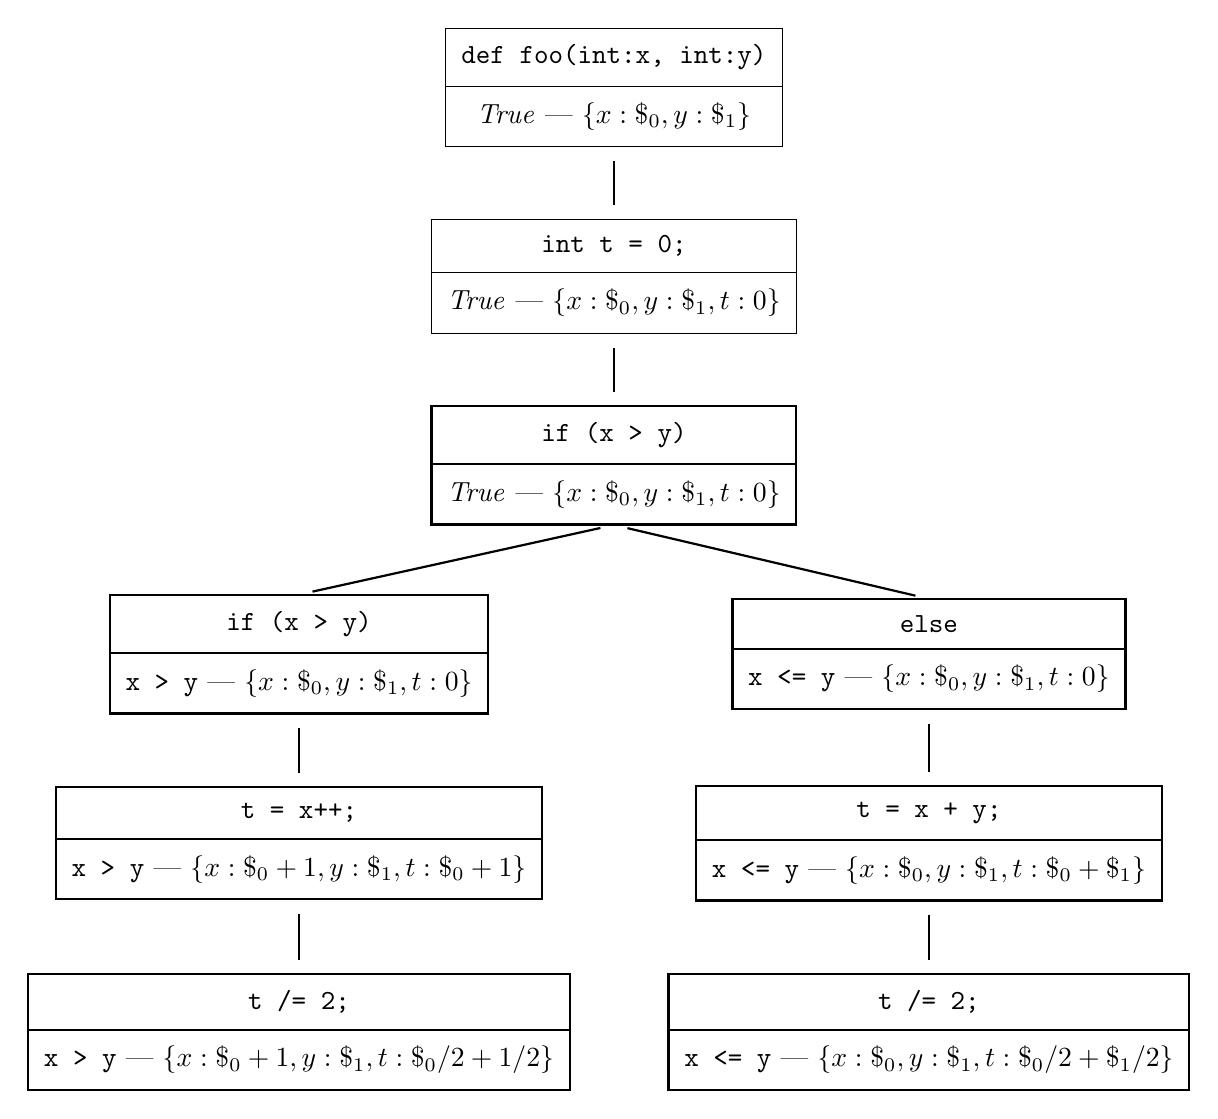
\begin{tikzpicture}[
    grow=down,
    level 1/.style={sibling distance=8cm,level distance=2.4cm},
    edge from parent/.style={thick,draw=black, shorten >=5pt, shorten <=5pt},
    edge from parent path={(\tikzparentnode.south) -- (\tikzchildnode.north)},
    kant/.style={text width=2cm, text centered, sloped},
    every node/.style={inner sep=2mm},
    punkt/.style={rectangle, top color=white,
    bottom color=white, draw=black}
]

\node[punkt] [rectangle split, rectangle split parts=2] {
    \texttt{def foo(int:x, int:y)}
    \nodepart{second}
    \textit{True} |
    $\{x: \$_0, y: \$_1\}$
}
child {
node[punkt] [rectangle split, rectangle split parts=2] {
    \texttt{int t = 0;}
    \nodepart{second}
    \textit{True} |
    $\{x: \$_0, y: \$_1, t: 0\}$
}
child {
node[punkt] [rectangle split, rectangle split parts=2] {
    \texttt{if (x > y)}
    \nodepart{second}
    \textit{True} |
    $\{x: \$_0, y: \$_1, t: 0\}$
}
    child {
        node[punkt] [rectangle split, rectangle split parts=2] {
            \texttt{if (x > y)}
            \nodepart{second}
            \texttt{x > y} |
            $\{x: \$_0, y: \$_1, t: 0\}$
        }
        child {
            node[punkt] [rectangle split, rectangle split parts=2] {
                \texttt{t = x++;}
                \nodepart{second}
                \texttt{x > y} |
                $\{x: \$_0+1, y: \$_1, t: \$_0+1\}$
            }
            child {
                node[punkt] [rectangle split, rectangle split parts=2] {
                    \texttt{t /= 2;}
                    \nodepart{second}
                    \texttt{x > y} |
                    $\{x: \$_0+1, y: \$_1, t: \$_0/2+1/2\}$
                }
            }
        }
    }
    child {
        node[punkt] [rectangle split, rectangle split parts=2] {
            \texttt{else}
            \nodepart{second}
            \texttt{x <= y} |
            $\{x: \$_0, y: \$_1, t: 0\}$
        }
        child {
            node[punkt] [rectangle split, rectangle split parts=2] {
                \texttt{t = x + y;}
                \nodepart{second}
                \texttt{x <= y} |
                $\{x: \$_0, y: \$_1, t: \$_0+\$_1 \}$
            }
            child {
                node[punkt] [rectangle split, rectangle split parts=2] {
                    \texttt{t /= 2;}
                    \nodepart{second}
                    \texttt{x <= y} |
                    $\{x: \$_0, y: \$_1, t: \$_0/2+\$_1/2\}$
                }
            }
        }
    }
}
};
\end{tikzpicture}\\

In order to generate such a tree, the \texttt{simulateExecution} method pops the statement on top of the stack, and it checks whether it is a concrete statement or a meta-instruction. In the first case we need to detect the statement type and simulate its behavior. One or more child states are created (based on the type of statement), and after setting them up (as well as the execution stack, if it needs to be modified) there is a recursive call for each of the child states. The base case occurs when the execution stack is empty, in which case the qubit upper bound is checked against the information that the \texttt{QRegManager} holds.
Now we describe the operations of the symbolic execution engine for each statement type.

\subsection{Expression statements}
The simulation of expression statements, just like the majority of the others, starts with the cloning of the current state. The expression statement can only modify the state if incrementors are present (i.e. \texttt{++} or \texttt{--}). The expression node is passed to the \texttt{Expression} constructor, and an evaluation is performed on the store of the new state. Since the evaluation procedure automatically updates the values of variables in the store if incrementors are found, the simulation is over after the evaluation. The final value of the expression is discarded, and the engine can proceed with the execution of the next statement.
\subsection{Assignment statements}
There are two types of assignment statements: classical ones and quantum measurements.
\subsubsection{Classical assignments}
Classical assignments involve a LHS (Left-Hand Side) and a RHS (Right-Hand Side) expressions. The RHS can be either an expression or an index identifier. In the first case it is evaluated to a symbolic expression, while in the second case it becomes a \texttt{CReg}. The assignment operator can include a binary operator (e.g. \texttt{+=}, \texttt{-=}, etc.), in which case the LHS is also evaluated and the binary operator is applied to the couple (LHS, RHS).
The final step is setting the value in the store, which is done by calling its \texttt{assign} method. If the old value in the store is a simple symbolic expression, it is just overwritten, but if it is a \texttt{CReg}, its \texttt{content} array is updated according to the new value.
\subsubsection{Quantum measurements}
Quantum measurements return a fresh symbol and set it in the store, since we ignore what happens at quantum level. Furthermore, when a quantum measurement is performed, the measured qubits and all the ones entangled to them are transfered by the \texttt{QRegManager} from the \texttt{potentialEntanglements} array to the \texttt{effectiveQubits} set by invoking the \texttt{markAsMeasured} method.

\subsection{Classical declarations}
The main difference between declarations and assignments is that the first have to take the type and domain of the variable into account. This is accomplished by calling the \texttt{ClassicalType} class constructor with the arguments obtained by inspecting the statement subtree.\\
Since declaration can have an immediate assignment, that case is handled like the corresponding statement, after having initialized the store item with the correct type.\\
Constant declarations are allowed too, but the type does not need to be specified. Thus, the store item will only contain the `value' field, and this is fine because the type is only needed when treating symbols with the SMT solver.

\subsection{Branching statements}
When simulating if-then-else statements, both paths need to be generated, unless one of them has an unsatisfiable condition. In other words, the first thing to do is evaluate the boolean expression of the condition and check both it and its negation for unsatisfiability. If one of them is unsatisfiable, the corresponding path is not generated.\\
Once determined which paths are to be generated, a clone state and a clone execution stack is created for each one of them, and the corresponding program blocks are expanded into sequences of statements and pushed on top of their execution stack. This is necessary because a branching instruction hides all the statements that are in the nested blocks, and so they need to be explicitly pushed on the stack for the engine to execute them. Notice that the statements that appear after the end of the if-then-else remain untouched and are present in all the execution stack's clones, just below the expanded blocks.\\
All child states are appended to the current state's \texttt{children} array, and a recursive call to the \texttt{simulateExecution} method is done for each one of them, with the corresponding execution stack passed as second argument.


\subsection{Quantum statements}
When a quantum gate call is encountered, all the qubits that appear in the it are considered to be potentially entangled, so the \texttt{addPotentialEntanglement} method of \texttt{QRegManager} is called on them.
\begin{example}
Suppose we have the following quantum registers:
\begin{lstlisting}
qreg q[4];
qreg r[4];
qreg s[4];
\end{lstlisting}
Here is an example of how the \texttt{QRegManager} arrays are affected by quantum statements (we put the array contents as comments between statements):
\begin{lstlisting}
// potentialEntanglements: []
// effectiveQubits: []

CX q[0], q[1];

// potentialEntanglements: [ {q[0],q[1]} ]
// effectiveQubits: []

CX q[2], r[0];

// potentialEntanglements: [ {q[0],q[1]}, {q[2],r[0]} ]
// effectiveQubits: []

CX q[1], q[3];

// potentialEntanglements: [ {q[0],q[1],q[3]}, {q[2],r[0]} ]
// effectiveQubits: []

CX r[1:4], s[1:4];

// potentialEntanglements: [ {q[0],q[1],q[3]}, {q[2],r[0]},
//     {r[1],s[1]}, {r[2],s[2]}, {r[3],s[3]} ]
// effectiveQubits: []

CX r[2], r[3];

// potentialEntanglements: [ {q[0],q[1],q[3]}, {q[2],r[0]},
//     {r[1],s[1]}, {r[2],s[2],r[3],s[3]} ]
// effectiveQubits: []

CX r[0], s[3];

// potentialEntanglements: [ {q[0],q[1],q[3]},
//     {q[2],r[0],r[2],s[2],r[3],s[3]}, {r[1],s[1]} ]
// effectiveQubits: []

measure r[2];

// potentialEntanglements: [ {q[0],q[1],q[3]}, {r[1],s[1]} ]
// effectiveQubits: [ q[2],r[0],r[2],s[2],r[3],s[3] ]

measure q[0];

// potentialEntanglements: [ {r[1],s[1]} ]
// effectiveQubits: [ q[2],r[0],r[2],s[2],r[3],s[3],q[0],
//     q[1],q[3] ]
\end{lstlisting}
The code above uses only 9 qubits (the size of \texttt{effectiveQubits} array) out of 12 that have been declared. The QASM analyzer is therefore able to tell the programmer which qubits are effectively used, so that resources can be saved for other computations.
\end{example}
\subsection{Loop statements}
Simulating loops symbolically is a hard task, so in this version of the analyzer only `for' loops with a known number of iterations have been considered. When such a loop statement is encountered, the execution stack is updated so that the loop block is repeated the correct number of times, and between two consecutive sequences there is a \texttt{SetStoreValueInstruction} that updates the value of the iterator.
\begin{example}
Suppose we have the following `for' loop.
\begin{lstlisting}
for i in [0:4] {
    CX q[i], r[i];
    c[i] = measure r[i];
}
\end{lstlisting}
Suppose also that the execution stack is already filled with some statements and the \texttt{for} loop on the top.\\
\\
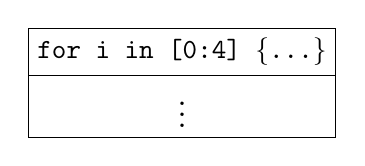
\begin{tikzpicture}[stack/.style={rectangle split, rectangle split parts=#1,draw, anchor=center}]
    \node[stack=2]  {\texttt{for i in [0:4] \{\ldots\}}
    \nodepart{two}\texttt{$\vdots$}
    };
\end{tikzpicture}
\\
So, when the engine simulates the \texttt{for} statement, the execution stack becomes:\\
\\
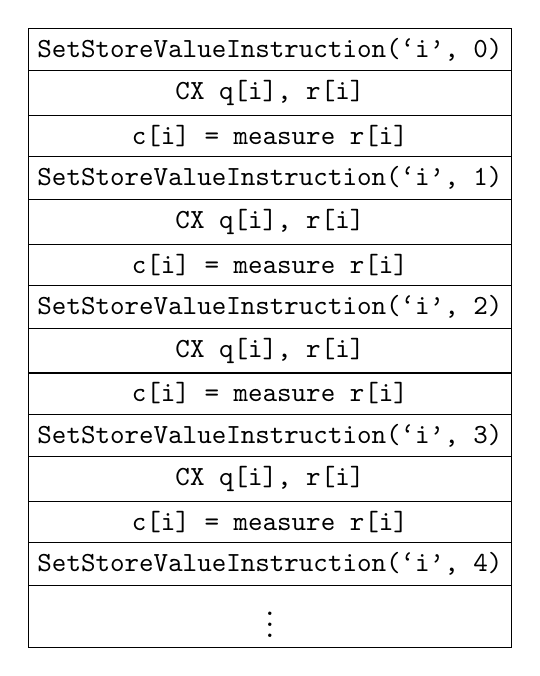
\begin{tikzpicture}[stack/.style={rectangle split, rectangle split parts=#1,draw, anchor=center}]
    \node[stack=14]  {
        \texttt{SetStoreValueInstruction(`i', 0)}
    \nodepart{two}\texttt{CX q[i], r[i]}
    \nodepart{three}\texttt{c[i] = measure r[i]}
    \nodepart{four}\texttt{SetStoreValueInstruction(`i', 1)}
    \nodepart{five}\texttt{CX q[i], r[i]}
    \nodepart{six}\texttt{c[i] = measure r[i]}
    \nodepart{seven}\texttt{SetStoreValueInstruction(`i', 2)}
    \nodepart{eight}\texttt{CX q[i], r[i]}
    \nodepart{nine}\texttt{c[i] = measure r[i]}
    \nodepart{ten}\texttt{SetStoreValueInstruction(`i', 3)}
    \nodepart{eleven}\texttt{CX q[i], r[i]}
    \nodepart{twelve}\texttt{c[i] = measure r[i]}
    \nodepart{thirteen}\texttt{SetStoreValueInstruction(`i', 4)}
    \nodepart{fourteen}\texttt{$\vdots$}

    };
\end{tikzpicture}
\end{example}
\section{Limitations and future development}
% todos and undetermined loops with assertions
There are some features that have not been implemented in this simple version of QASM analyzer, such as:
\begin{itemize}
    \itemsep 0em
    \item Function calls in expressions (e.g. \texttt{2 + a + getNumber()})
    \item Boolean auto-cast in conditional statements (e.g. \texttt{if (variable)}): the libraries make it hard to cast from number to boolean.
    \item Bitwise shift operations (\texttt{<<} and \texttt{>>}): bit vectors are only available in \texttt{PySMT}, not in \texttt{sympy}.
    \item Modulo operation (\texttt{\%}): not available in \texttt{PySMT}
    \item Alias statements (e.g. \texttt{let y = x}): keeping track of all the references could be difficult, especially if there are more levels of indirection.
    \item Indeterminate loops (e.g. \texttt{while (a > 0)}): here some technique should be used to detect loop invariants and use them to make assertions about pre- and post-conditions.
    \item Control directive statements (\texttt{break}, \texttt{continue} and \texttt{end}): they would complicate indeterminate loop handling even more.
    \item Symbolic designators in index identifiers (e.g. \texttt{a[n]}, where \texttt{n} is not known at compile time): every time a symbolic designator is detected, it should be checked against all the previous ones and check for equalities. This is quite time-consuming and it does not always guarantee that the analysis is correct.
\end{itemize}
In conclusion, we could say that this is the first version of a static analyzer for QASM, and the main concern is to estimate the number of qubits that are measured and/or entangled to measured ones. This could help quantum programmers to care about the resources that they use, and this is fundamental in quantum computing since qubits are really expensive, and the real power of quantum superpositions, that allow multiple states to be computed at the same time, is exponential with respect to the number of qubits.\\

\section{Conclusion}
The path for Quantum Supremacy is still long, but every step counts. Reducing the number of qubits that a program requires is a tiny step, but together with other innovations and newer technologies for the physical implementation of qubits, could make the difference and lead to a completely new scenario for communications, cryptography, big data and simulations of chemicals and phisical phenomena.

\printbibliography
\end{document}